% Options for packages loaded elsewhere
\PassOptionsToPackage{unicode}{hyperref}
\PassOptionsToPackage{hyphens}{url}
%
\documentclass[
  ignorenonframetext,
]{beamer}
\usepackage{pgfpages}
\setbeamertemplate{caption}[numbered]
\setbeamertemplate{caption label separator}{: }
\setbeamercolor{caption name}{fg=normal text.fg}
\beamertemplatenavigationsymbolsempty
% Prevent slide breaks in the middle of a paragraph
\widowpenalties 1 10000
\raggedbottom
\setbeamertemplate{part page}{
  \centering
  \begin{beamercolorbox}[sep=16pt,center]{part title}
    \usebeamerfont{part title}\insertpart\par
  \end{beamercolorbox}
}
\setbeamertemplate{section page}{
  \centering
  \begin{beamercolorbox}[sep=12pt,center]{part title}
    \usebeamerfont{section title}\insertsection\par
  \end{beamercolorbox}
}
\setbeamertemplate{subsection page}{
  \centering
  \begin{beamercolorbox}[sep=8pt,center]{part title}
    \usebeamerfont{subsection title}\insertsubsection\par
  \end{beamercolorbox}
}
\AtBeginPart{
  \frame{\partpage}
}
\AtBeginSection{
  \ifbibliography
  \else
    \frame{\sectionpage}
  \fi
}
\AtBeginSubsection{
  \frame{\subsectionpage}
}

\usepackage{amsmath,amssymb}
\usepackage{iftex}
\ifPDFTeX
  \usepackage[T1]{fontenc}
  \usepackage[utf8]{inputenc}
  \usepackage{textcomp} % provide euro and other symbols
\else % if luatex or xetex
  \usepackage{unicode-math}
  \defaultfontfeatures{Scale=MatchLowercase}
  \defaultfontfeatures[\rmfamily]{Ligatures=TeX,Scale=1}
\fi
\usepackage{lmodern}
\ifPDFTeX\else  
    % xetex/luatex font selection
\fi
% Use upquote if available, for straight quotes in verbatim environments
\IfFileExists{upquote.sty}{\usepackage{upquote}}{}
\IfFileExists{microtype.sty}{% use microtype if available
  \usepackage[]{microtype}
  \UseMicrotypeSet[protrusion]{basicmath} % disable protrusion for tt fonts
}{}
\makeatletter
\@ifundefined{KOMAClassName}{% if non-KOMA class
  \IfFileExists{parskip.sty}{%
    \usepackage{parskip}
  }{% else
    \setlength{\parindent}{0pt}
    \setlength{\parskip}{6pt plus 2pt minus 1pt}}
}{% if KOMA class
  \KOMAoptions{parskip=half}}
\makeatother
\usepackage{xcolor}
\newif\ifbibliography
\setlength{\emergencystretch}{3em} % prevent overfull lines
\setcounter{secnumdepth}{-\maxdimen} % remove section numbering


\providecommand{\tightlist}{%
  \setlength{\itemsep}{0pt}\setlength{\parskip}{0pt}}\usepackage{longtable,booktabs,array}
\usepackage{calc} % for calculating minipage widths
\usepackage{caption}
% Make caption package work with longtable
\makeatletter
\def\fnum@table{\tablename~\thetable}
\makeatother
\usepackage{graphicx}
\makeatletter
\def\maxwidth{\ifdim\Gin@nat@width>\linewidth\linewidth\else\Gin@nat@width\fi}
\def\maxheight{\ifdim\Gin@nat@height>\textheight\textheight\else\Gin@nat@height\fi}
\makeatother
% Scale images if necessary, so that they will not overflow the page
% margins by default, and it is still possible to overwrite the defaults
% using explicit options in \includegraphics[width, height, ...]{}
\setkeys{Gin}{width=\maxwidth,height=\maxheight,keepaspectratio}
% Set default figure placement to htbp
\makeatletter
\def\fps@figure{htbp}
\makeatother

\makeatletter
\makeatother
\makeatletter
\makeatother
\makeatletter
\@ifpackageloaded{caption}{}{\usepackage{caption}}
\AtBeginDocument{%
\ifdefined\contentsname
  \renewcommand*\contentsname{Table of contents}
\else
  \newcommand\contentsname{Table of contents}
\fi
\ifdefined\listfigurename
  \renewcommand*\listfigurename{List of Figures}
\else
  \newcommand\listfigurename{List of Figures}
\fi
\ifdefined\listtablename
  \renewcommand*\listtablename{List of Tables}
\else
  \newcommand\listtablename{List of Tables}
\fi
\ifdefined\figurename
  \renewcommand*\figurename{Figure}
\else
  \newcommand\figurename{Figure}
\fi
\ifdefined\tablename
  \renewcommand*\tablename{Table}
\else
  \newcommand\tablename{Table}
\fi
}
\@ifpackageloaded{float}{}{\usepackage{float}}
\floatstyle{ruled}
\@ifundefined{c@chapter}{\newfloat{codelisting}{h}{lop}}{\newfloat{codelisting}{h}{lop}[chapter]}
\floatname{codelisting}{Listing}
\newcommand*\listoflistings{\listof{codelisting}{List of Listings}}
\makeatother
\makeatletter
\@ifpackageloaded{caption}{}{\usepackage{caption}}
\@ifpackageloaded{subcaption}{}{\usepackage{subcaption}}
\makeatother
\makeatletter
\@ifpackageloaded{tcolorbox}{}{\usepackage[skins,breakable]{tcolorbox}}
\makeatother
\makeatletter
\@ifundefined{shadecolor}{\definecolor{shadecolor}{rgb}{.97, .97, .97}}
\makeatother
\makeatletter
\makeatother
\makeatletter
\makeatother
\ifLuaTeX
  \usepackage{selnolig}  % disable illegal ligatures
\fi
\IfFileExists{bookmark.sty}{\usepackage{bookmark}}{\usepackage{hyperref}}
\IfFileExists{xurl.sty}{\usepackage{xurl}}{} % add URL line breaks if available
\urlstyle{same} % disable monospaced font for URLs
\hypersetup{
  pdftitle={Principal Component Analysis},
  hidelinks,
  pdfcreator={LaTeX via pandoc}}

\title{Principal Component Analysis}
\author{}
\date{}

\begin{document}
\frame{\titlepage}
\ifdefined\Shaded\renewenvironment{Shaded}{\begin{tcolorbox}[breakable, frame hidden, interior hidden, enhanced, borderline west={3pt}{0pt}{shadecolor}, sharp corners, boxrule=0pt]}{\end{tcolorbox}}\fi

\begin{frame}{What it does?}
\protect\hypertarget{what-it-does}{}
\end{frame}

\begin{frame}{How does it do it?}
\protect\hypertarget{how-does-it-do-it}{}
\end{frame}

\begin{frame}[fragile]{PCA in a view or coordinate rotation}
\protect\hypertarget{pca-in-a-view-or-coordinate-rotation}{}
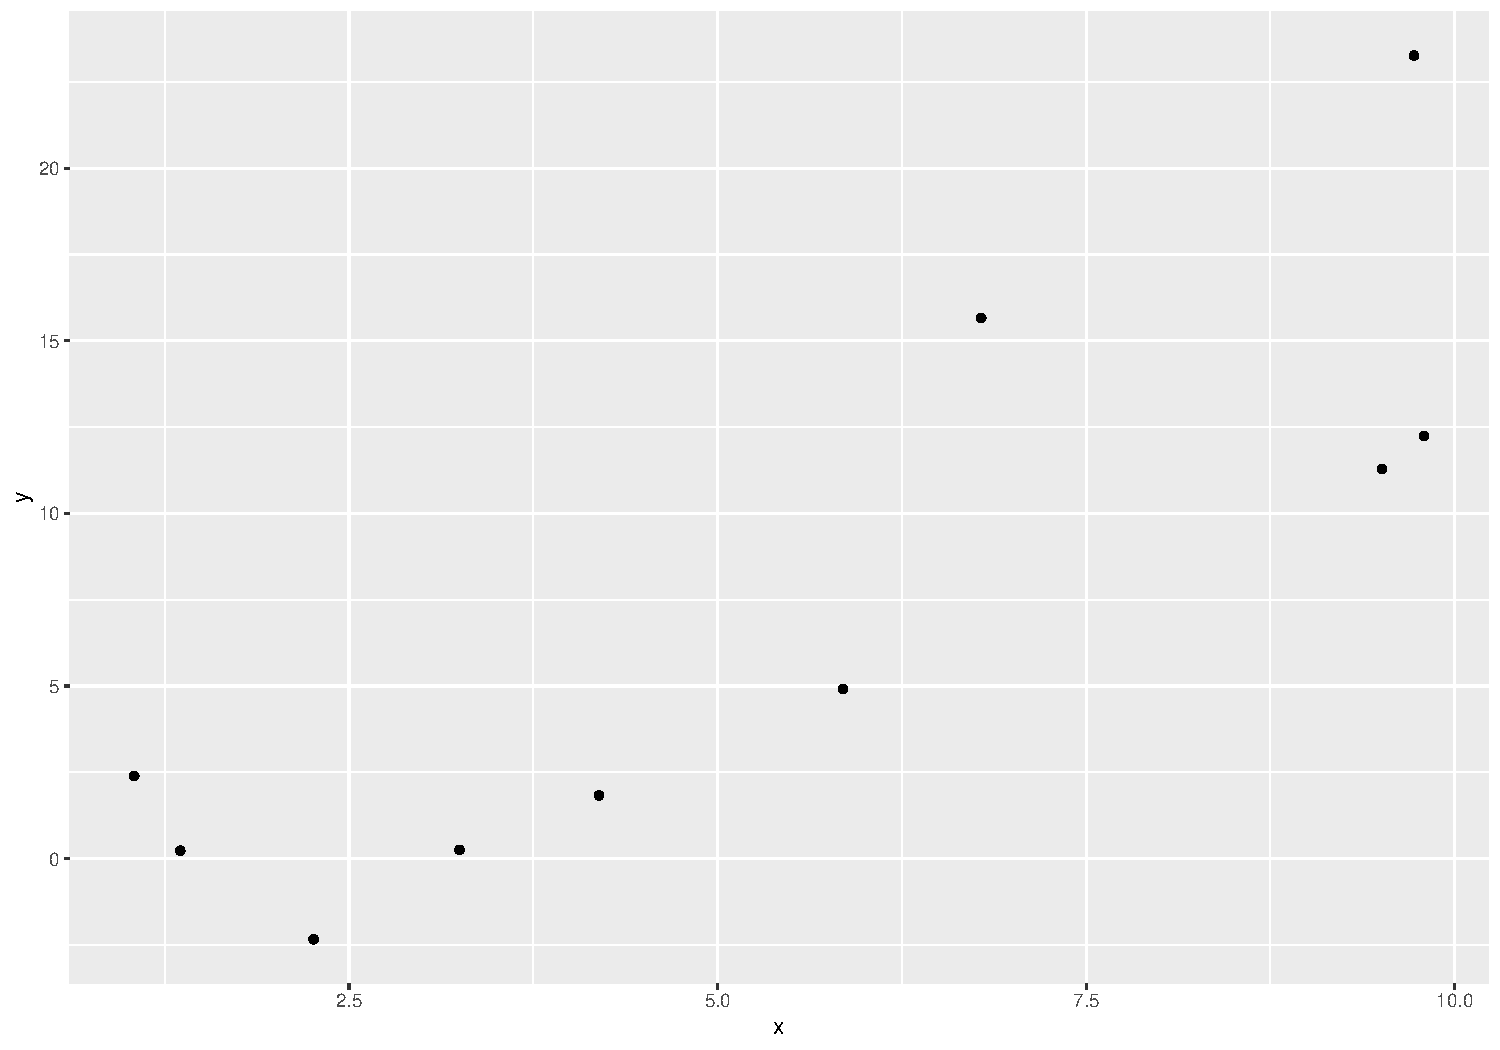
\includegraphics{note9_files/figure-beamer/unnamed-chunk-1-1.pdf}

\begin{verbatim}
Standard deviations (1, .., p=2):
[1] 8.802072 1.716667

Rotation (n x k) = (2 x 2):
          PC1        PC2
x1 -0.3490897 -0.9370893
x2 -0.9370893  0.3490897
\end{verbatim}

\begin{verbatim}
      eigenvalue variance.percent cumulative.variance.percent
Dim.1  77.476476        96.335712                    96.33571
Dim.2   2.946946         3.664288                   100.00000
\end{verbatim}

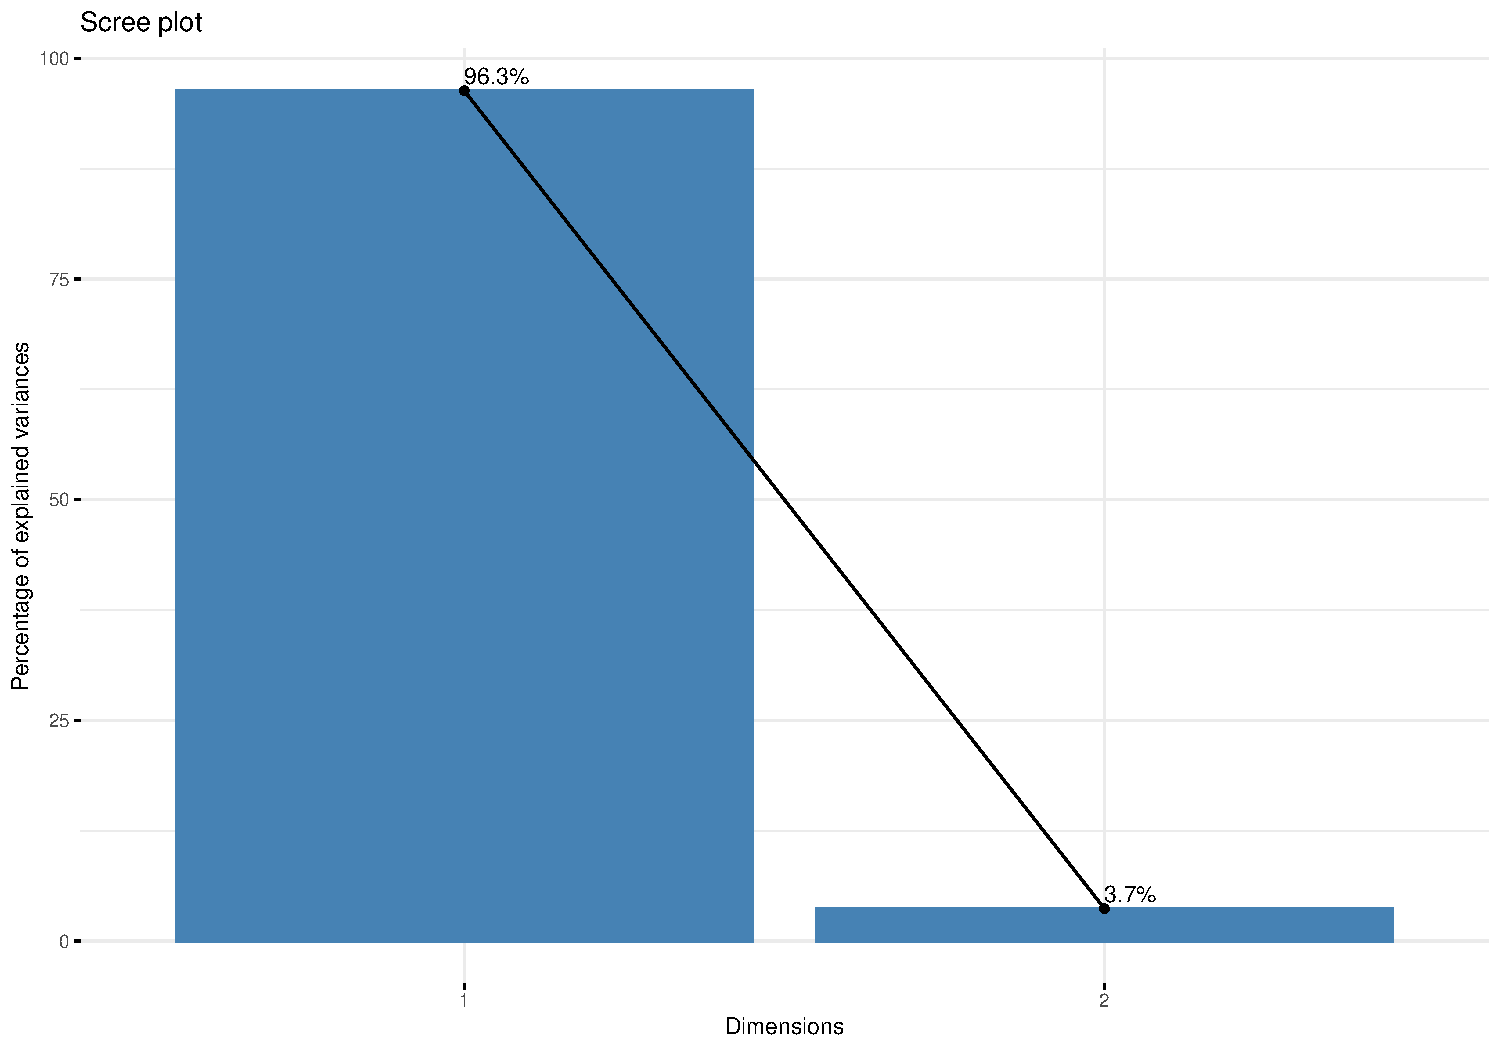
\includegraphics{note9_files/figure-beamer/unnamed-chunk-3-1.pdf}

\begin{itemize}
\tightlist
\item
  We notice that there are some information of salary in income
\item
  Could we combine this
\end{itemize}
\end{frame}

\begin{frame}{Another perspective of PCA}
\protect\hypertarget{another-perspective-of-pca}{}
\begin{itemize}
\item
  Consider \(n\) points of data. We look for a direction where the
  projections of these points to it give the maximum variance.
\item
  Projection of a point onto a direction (vector).
\item
  A point is presented by a pair of number \((3,4)\). A vector/direction
  is also presented by a pair of number: x-axis presented by \((1,0)\)
  and y-axis presented by \((0,1)\). A vector/direction of \((a,b)\)
  could be a point connecting the origin \((0,0)\) and the point
  \((a,b)\).
\item
  A projection of a point \((x_0, y_0)\) onto a vector \((a,b)\) is a
  number (scalar), it is the dot product of the two pair or
\end{itemize}

\[
ax_0 + by_0
\] - A vector also presents a subspace of one dimension. So we project a
point of two dimension onto a subspace of one dimension, the projection
should have only one number.
\end{frame}

\begin{frame}{PCA as projections onto subspace}
\protect\hypertarget{pca-as-projections-onto-subspace}{}
\begin{itemize}
\item
  If we have \(n\) points to a vector (one dimensional subspace), we
  will receive n numbers. Thus, a data of \(n\) points in two dimension
  (a pair), presented by a matrix, will turn into \(n\) numbers. So we
  can say that a matrix of \(n \times 2\), projected onto a vector will
  be \(n\) numbers (\(n\) points in one dimensional subspace).
\item
  So, \(n\) points projects onto a vector becomes \(n\) numbers. We want
  to find a vector/subspace that maximize the variance of this points.
  What is the variance of points. If the points have zero means, the
  variance is the length of the \(n\) points.
\item
  Language of subspace and projection and the language of statistics. We
  should discuss this using one language only.
\end{itemize}
\end{frame}

\begin{frame}{Projection of a point to a direction}
\protect\hypertarget{projection-of-a-point-to-a-direction}{}
\begin{itemize}
\item
  For simplicity, we first consider 2 dimension first
\item
  Both a point A and a vector OA (O is the origin) is presented by a
  column vector.
\item
  The projection of a point A, presented by a column vector
  \(b = [b_1, b_2]^T\) onto a vector through the origin, also presented
  by a column vector, \(a = [a_1, a_2]^T\) (or the span of this vector
  which is a 1-dimensional subspace) is
\end{itemize}

\[
\frac{aa^T}{a^Ta}b
\],
\end{frame}

\begin{frame}{Projection of a point to a direction}
\protect\hypertarget{projection-of-a-point-to-a-direction-1}{}
\begin{itemize}
\tightlist
\item
  \(P=\frac{aa^T}{a^Ta}\) is called a projection matrix.
\end{itemize}

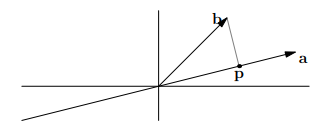
\includegraphics[width=2.51042in,height=\textheight]{images/pca1.png}

\begin{itemize}
\tightlist
\item
  For example, the projection of a point
  \(x = \begin{bmatrix} 1 \\ 3 \end{bmatrix}\) onto a direction of
  \(v = [3, 2]^T\) (or onto span(v)) is
\end{itemize}

\[
\frac{vv^T}{v^Tv}x = \begin{bmatrix}
   2.076923  \\ 1.384615
  \end{bmatrix}
\] - We usually consider the direction vector of length 1.
\end{frame}

\begin{frame}{Checking}
\protect\hypertarget{checking}{}
\begin{itemize}
\tightlist
\item
  Checking only.
\end{itemize}
\end{frame}

\begin{frame}{What does the \(v^Tx\) present?}
\protect\hypertarget{what-does-the-vtx-present}{}
\begin{itemize}
\item
  Sometime, the projection of a point
  \(x = \begin{bmatrix} 1 \\ 3 \end{bmatrix}\) onto \(span(v)\) where
  \(\|v\| = 1\) can be presented by a dot product \(x^Tv\).
\item
  This product is the length of the projected vector, which is also the
  coordinate of the projected point in a new axis \(v\).
\item
  This is because \[
  u = \frac{vv^T}{v^Tv}x = v\frac{v^Tx}{v^Tv} = vv^Tx \
  \implies \|u\| = \|v\|v^Tx = v^Tx
  \] as \(v^Tv = \|v\|^2=1\).
\end{itemize}
\end{frame}

\begin{frame}{Projections of \(n\) points to a direction}
\protect\hypertarget{projections-of-n-points-to-a-direction}{}
\begin{itemize}
\item
  The projection of vector \(x\) onto \(v\) is \(x^Tv\)
\item
  The projection \(n\) points
  \(X = \begin{bmatrix} x_1^T \\ x_2^T\\..\\x_n^T \end{bmatrix}\) (\(X\)
  is a \(n \times 2\) matrix) is
  \(Xv=\begin{bmatrix} x_1^Tv \\ x_2^Tv\\..\\x_n^Tv \end{bmatrix}\),
  which is a \(n \times 1\) matrix.
\item
  We can say that \(n\) points \(x_1^T, x_2^T,..., x_n^T\) in \(R^2\)
  are transformed to \(n\) points \(x_1^Tv, x_2^Tv,..., x_n^Tv\) in
  \(R^1\).
\end{itemize}
\end{frame}

\begin{frame}{Variance and Total Variance}
\protect\hypertarget{variance-and-total-variance}{}
\begin{itemize}
\item
  In one dimension, the variance of \(n\) points/numbers
  \(a_1, a_2,..., a_n\) is \(\frac{1}{n-1} \sum (a_i - \bar{a})^2\). If
  \(a\) is center, \(\bar{a}=0\), then the variance is
  \(\frac{1}{n-1} \sum a_i^2 = \frac{1}{n-1} \|a\|^2 = \frac{1}{n-1}a^Ta\).
\item
  Let \(X\) be an \(n \times 2\) data matrix. Let's X be centralized,
  which means both two columns have zero means. The projection of \(X\)
  onto \(v\), \(Xv\) also has zero mean. Thus, the variance of the
  projection \(Xv\) is \(\frac{1}{n-1} \|Xv\|^2\).
\item
  The total variance of the data is the sum of the variance of the
  projection onto the x-axis (var(x)) and the variance of the projection
  onto y-axis (var(y)).
\item
  If we rotate the xy axis into uv axis, the total variance does not
  change, var(u) + var(v) = var(x) + var(y)
\item
  PC1 is the direction that has the maximum variance of the data.
\end{itemize}
\end{frame}

\begin{frame}[fragile]{Demonstration}
\protect\hypertarget{demonstration}{}
\begin{verbatim}
[1] 26.21958
\end{verbatim}
\end{frame}

\begin{frame}{}
\protect\hypertarget{section}{}
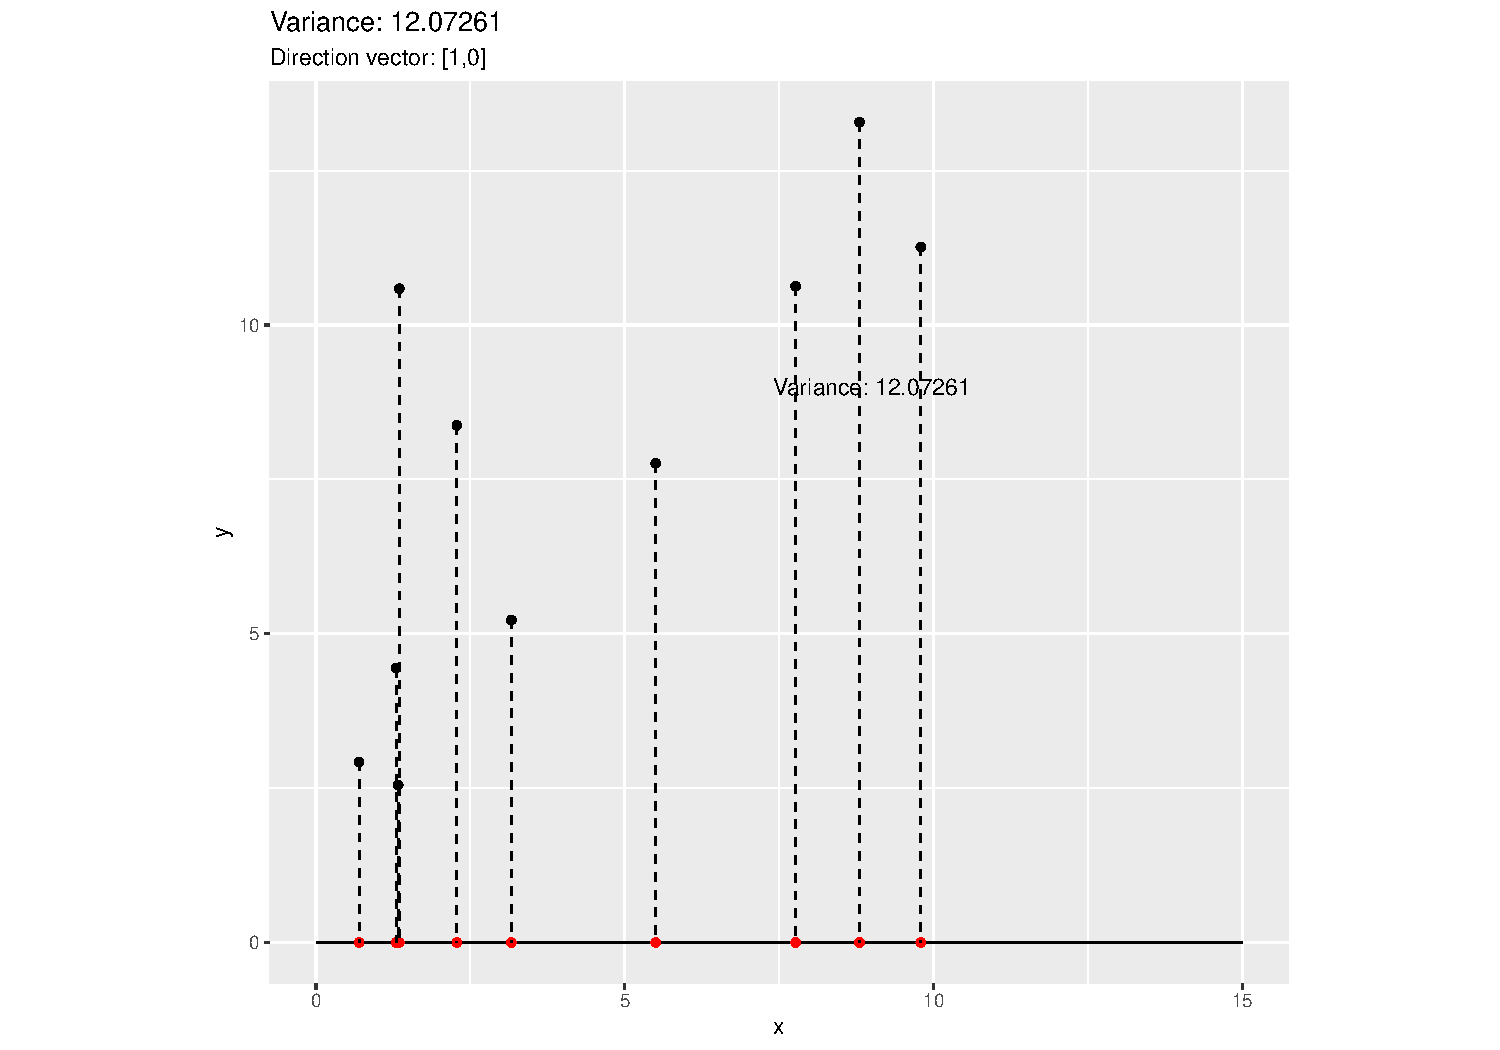
\includegraphics{note9_files/figure-beamer/unnamed-chunk-7-1.pdf}
\end{frame}

\begin{frame}{}
\protect\hypertarget{section-1}{}
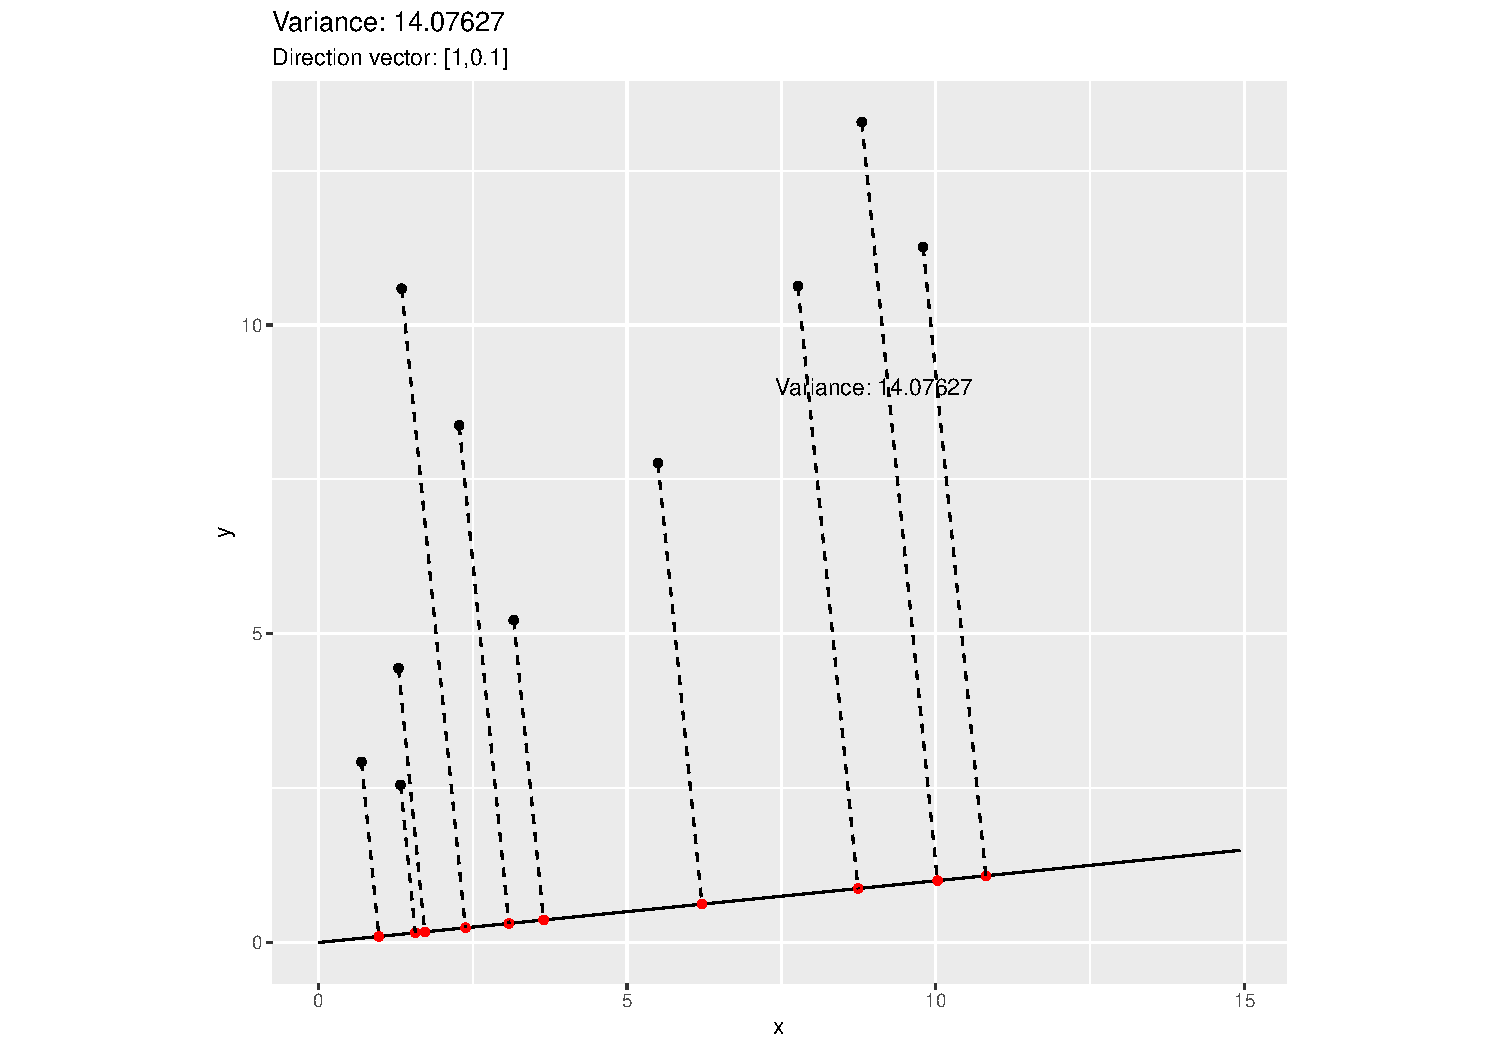
\includegraphics{note9_files/figure-beamer/unnamed-chunk-8-1.pdf}
\end{frame}

\begin{frame}{}
\protect\hypertarget{section-2}{}
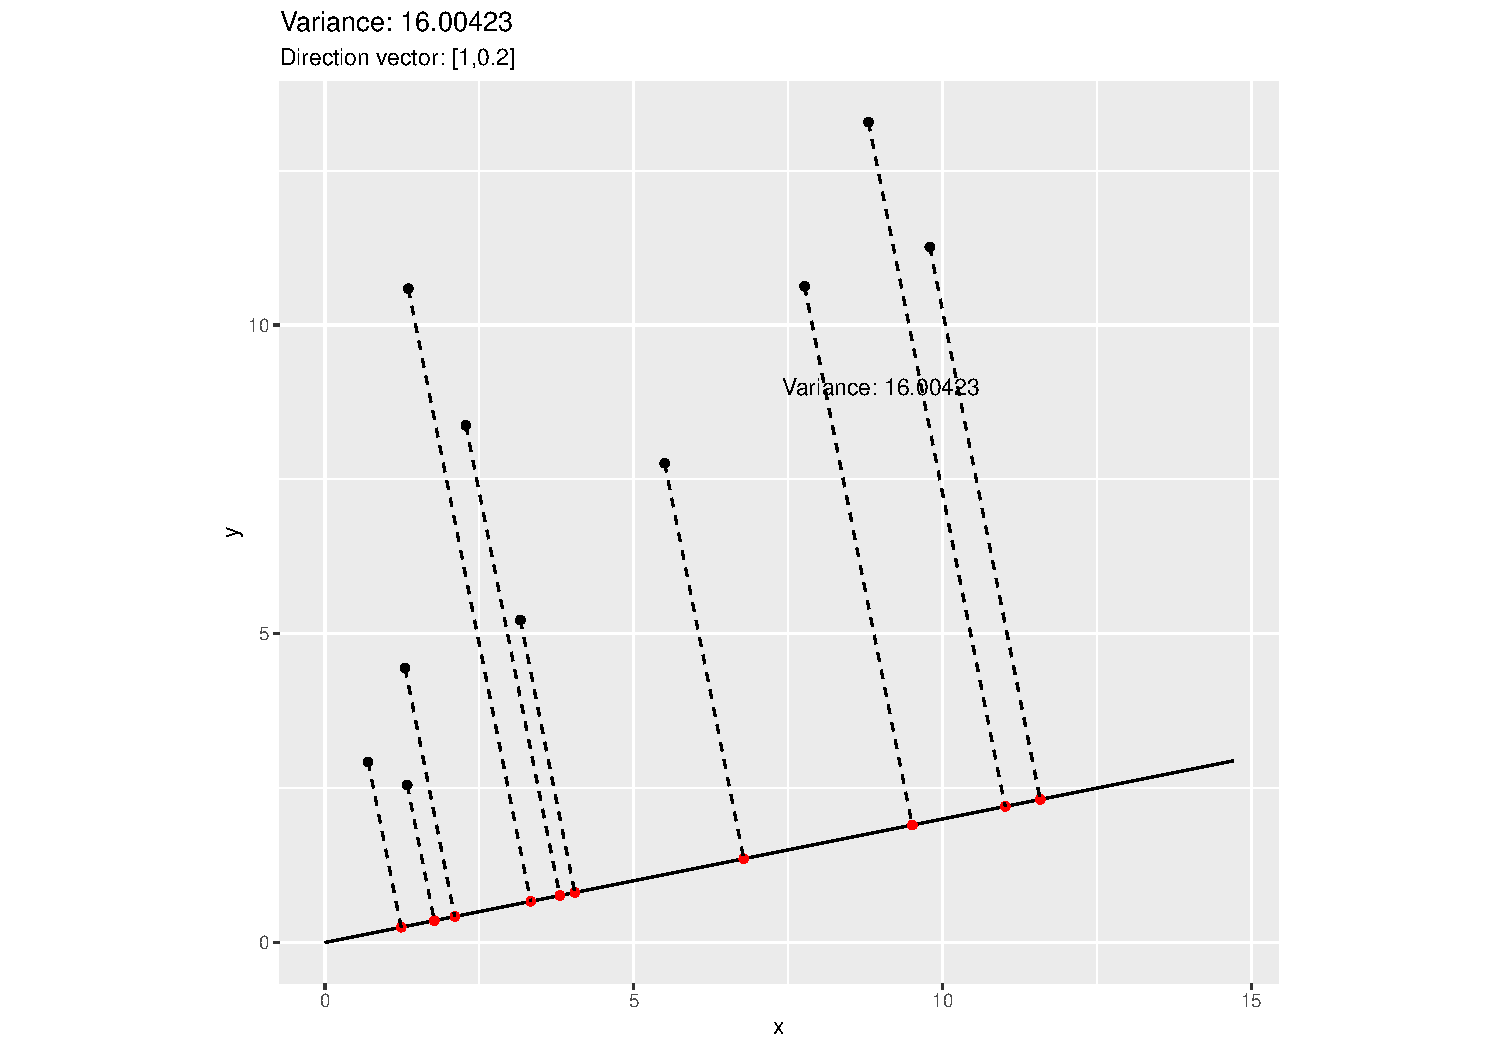
\includegraphics{note9_files/figure-beamer/unnamed-chunk-9-1.pdf}
\end{frame}

\begin{frame}{}
\protect\hypertarget{section-3}{}
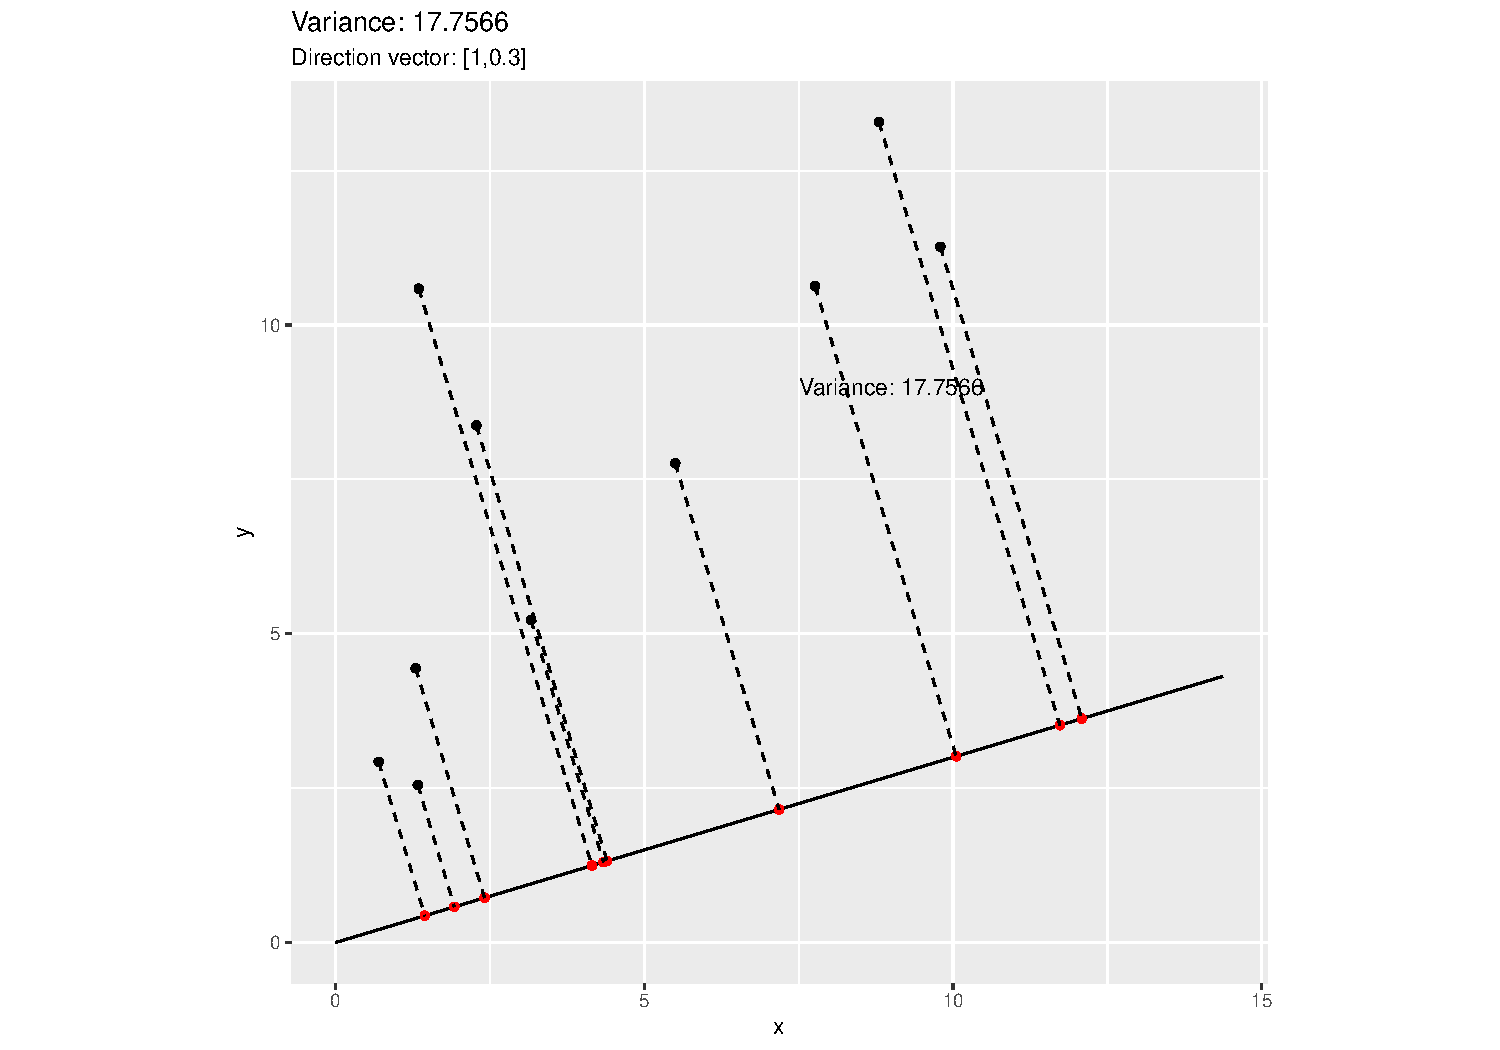
\includegraphics{note9_files/figure-beamer/unnamed-chunk-10-1.pdf}
\end{frame}

\begin{frame}{}
\protect\hypertarget{section-4}{}
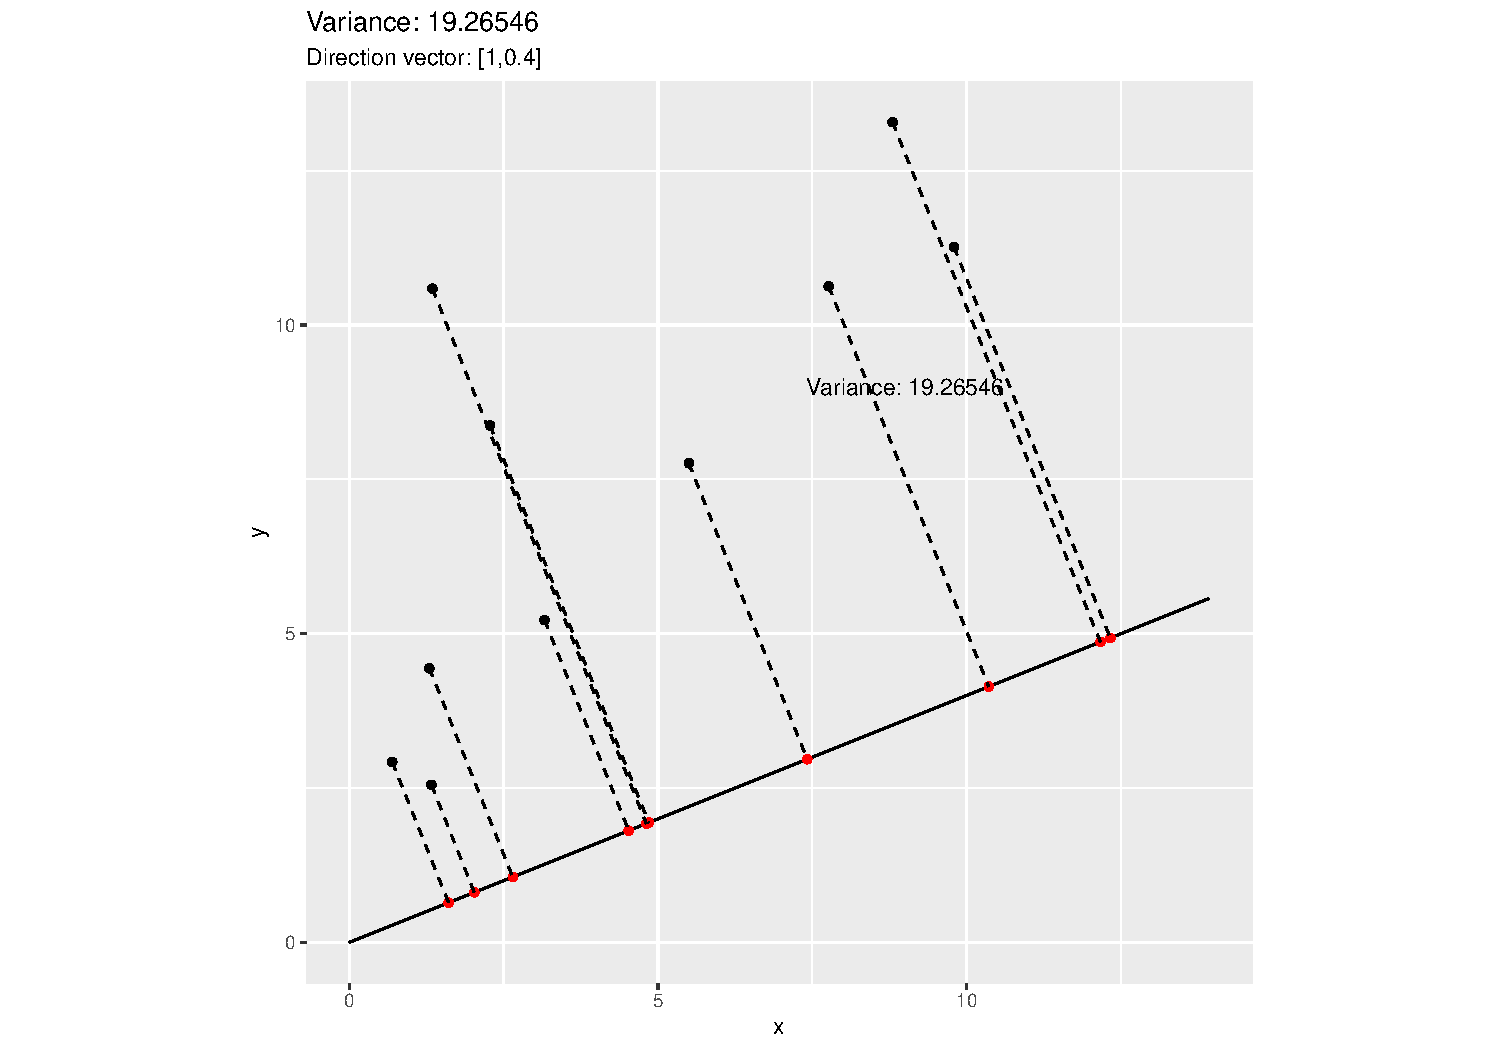
\includegraphics{note9_files/figure-beamer/unnamed-chunk-11-1.pdf}
\end{frame}

\begin{frame}{}
\protect\hypertarget{section-5}{}
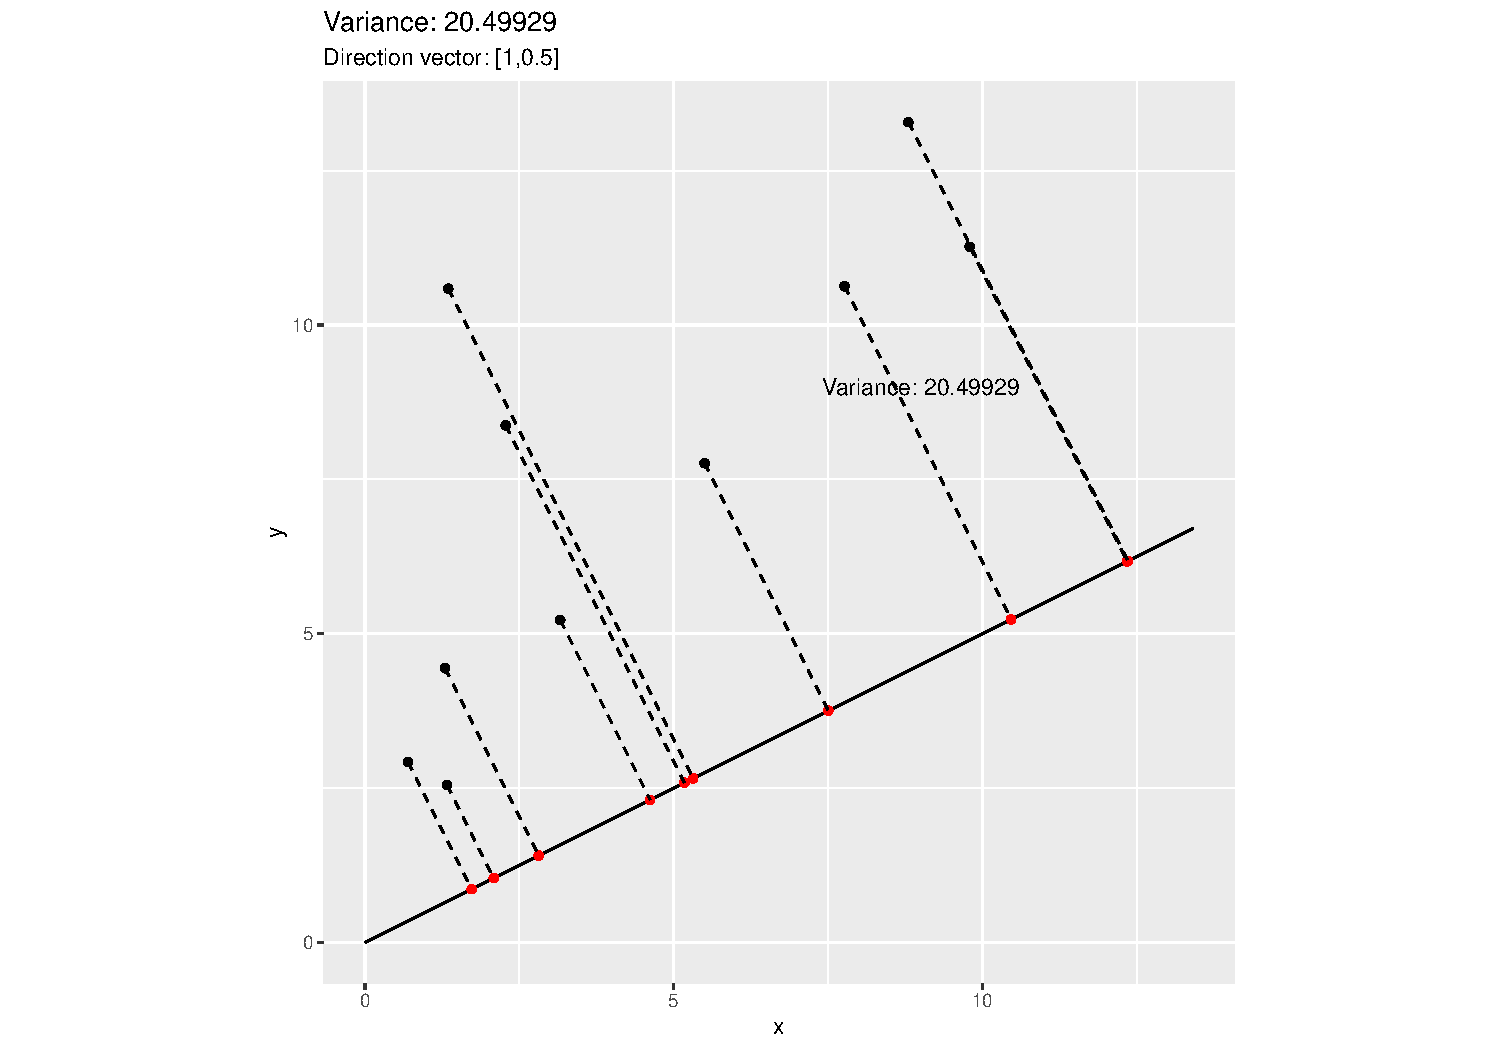
\includegraphics{note9_files/figure-beamer/unnamed-chunk-12-1.pdf}
\end{frame}

\begin{frame}{}
\protect\hypertarget{section-6}{}
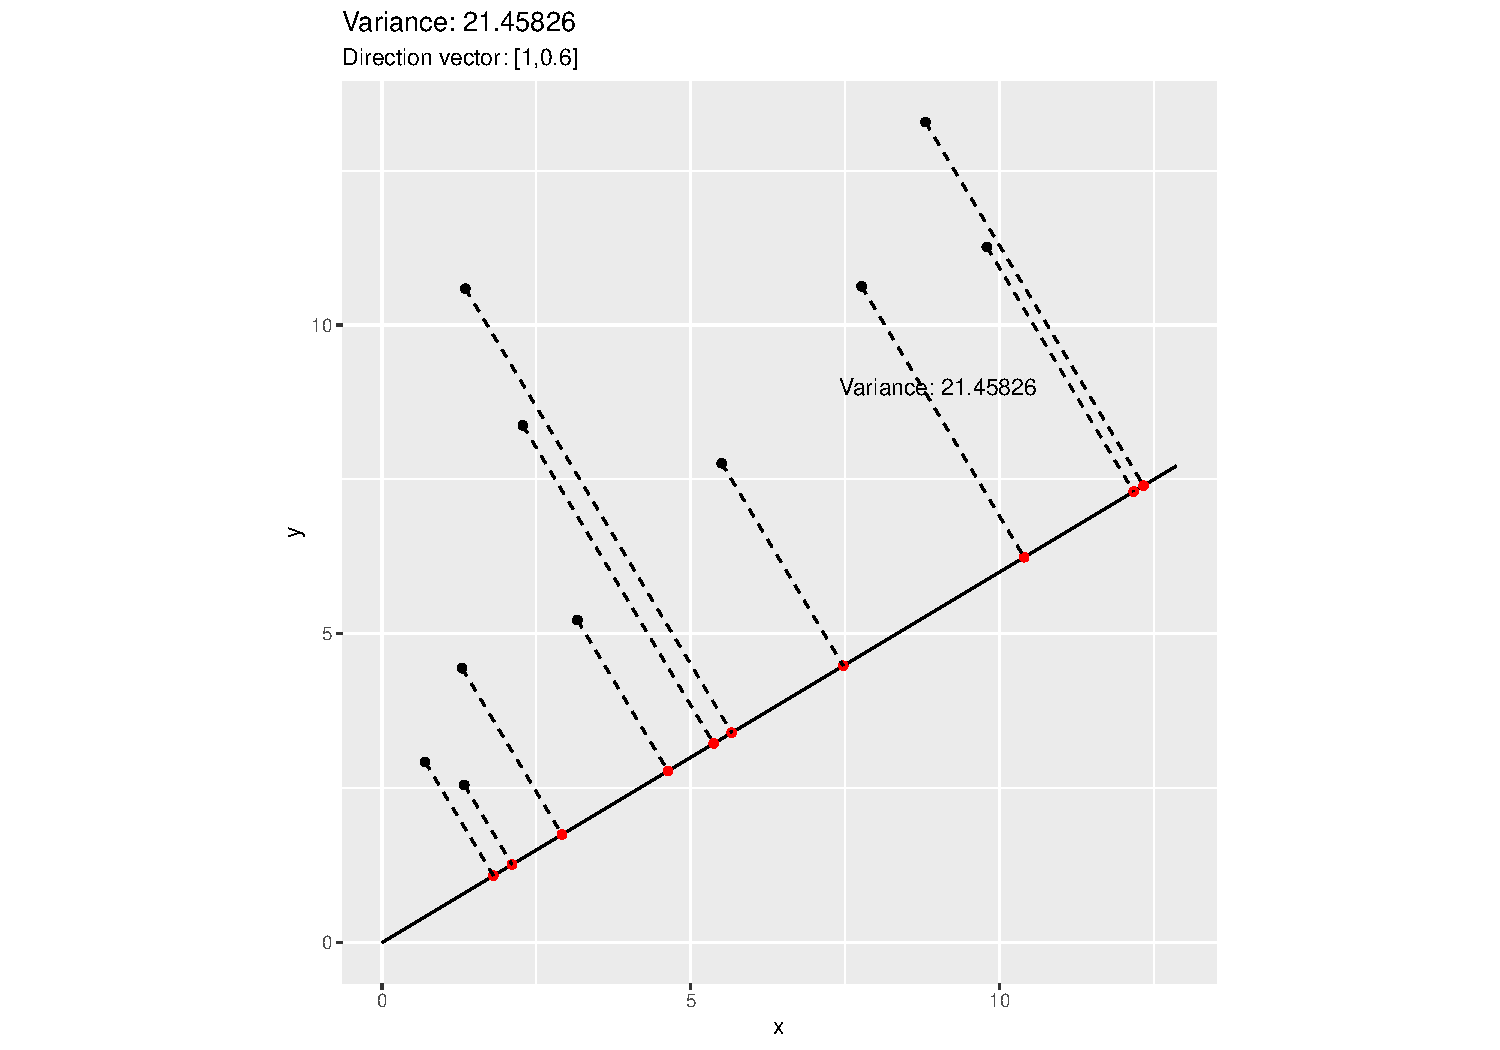
\includegraphics{note9_files/figure-beamer/unnamed-chunk-13-1.pdf}
\end{frame}

\begin{frame}{}
\protect\hypertarget{section-7}{}
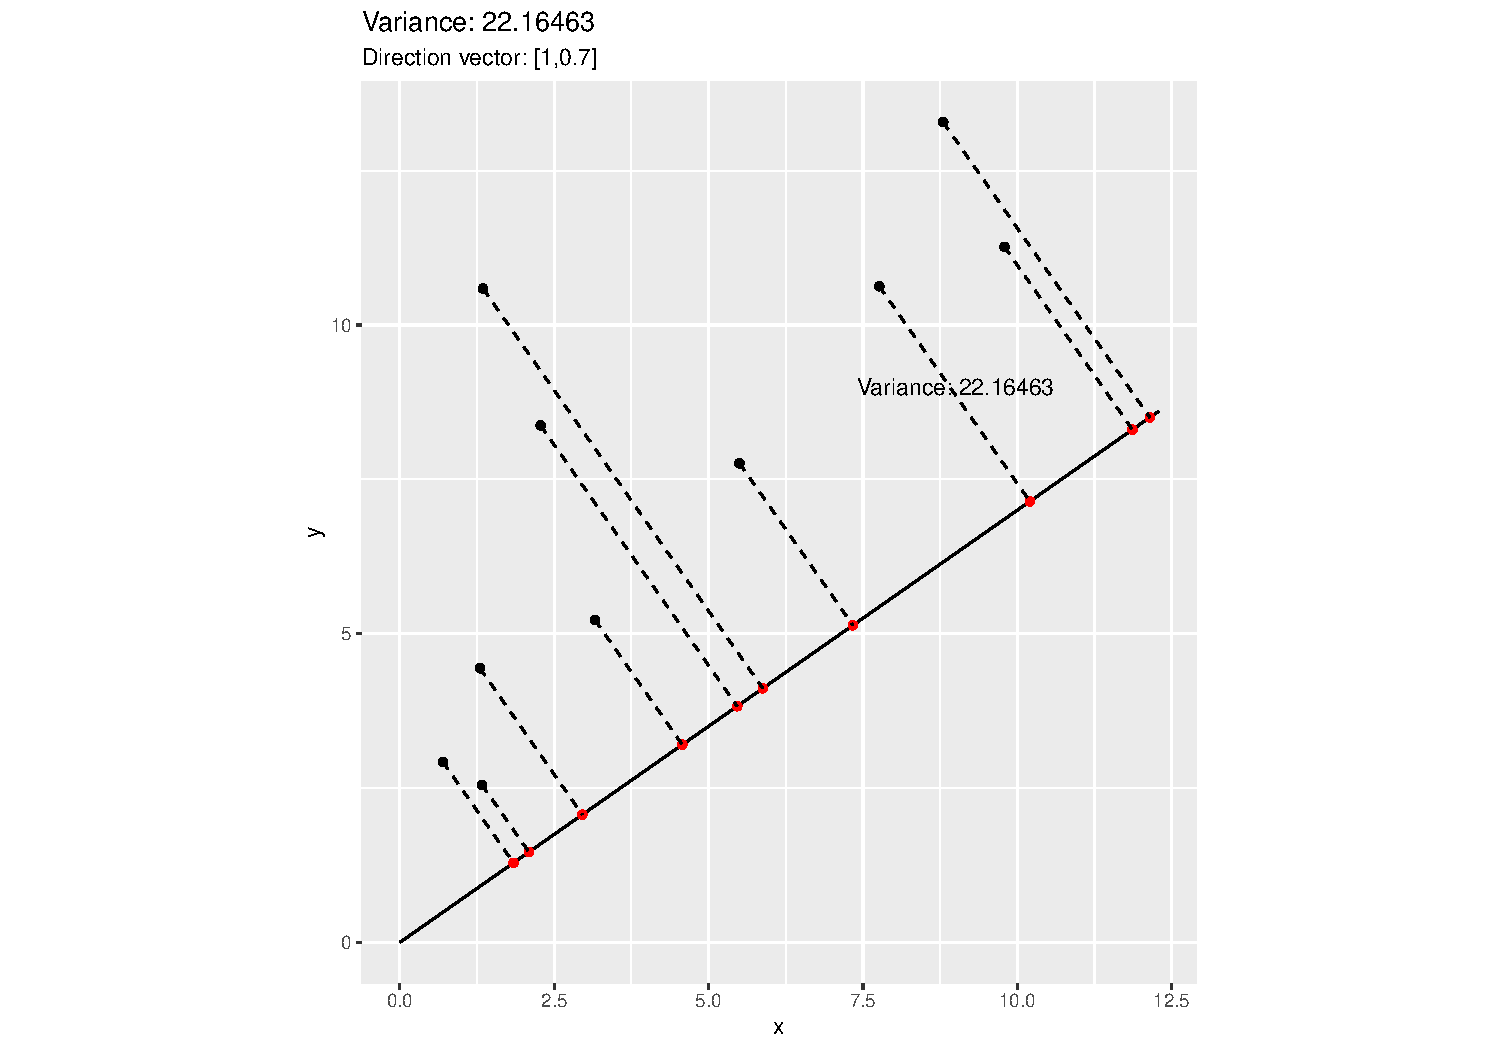
\includegraphics{note9_files/figure-beamer/unnamed-chunk-14-1.pdf}
\end{frame}

\begin{frame}{}
\protect\hypertarget{section-8}{}
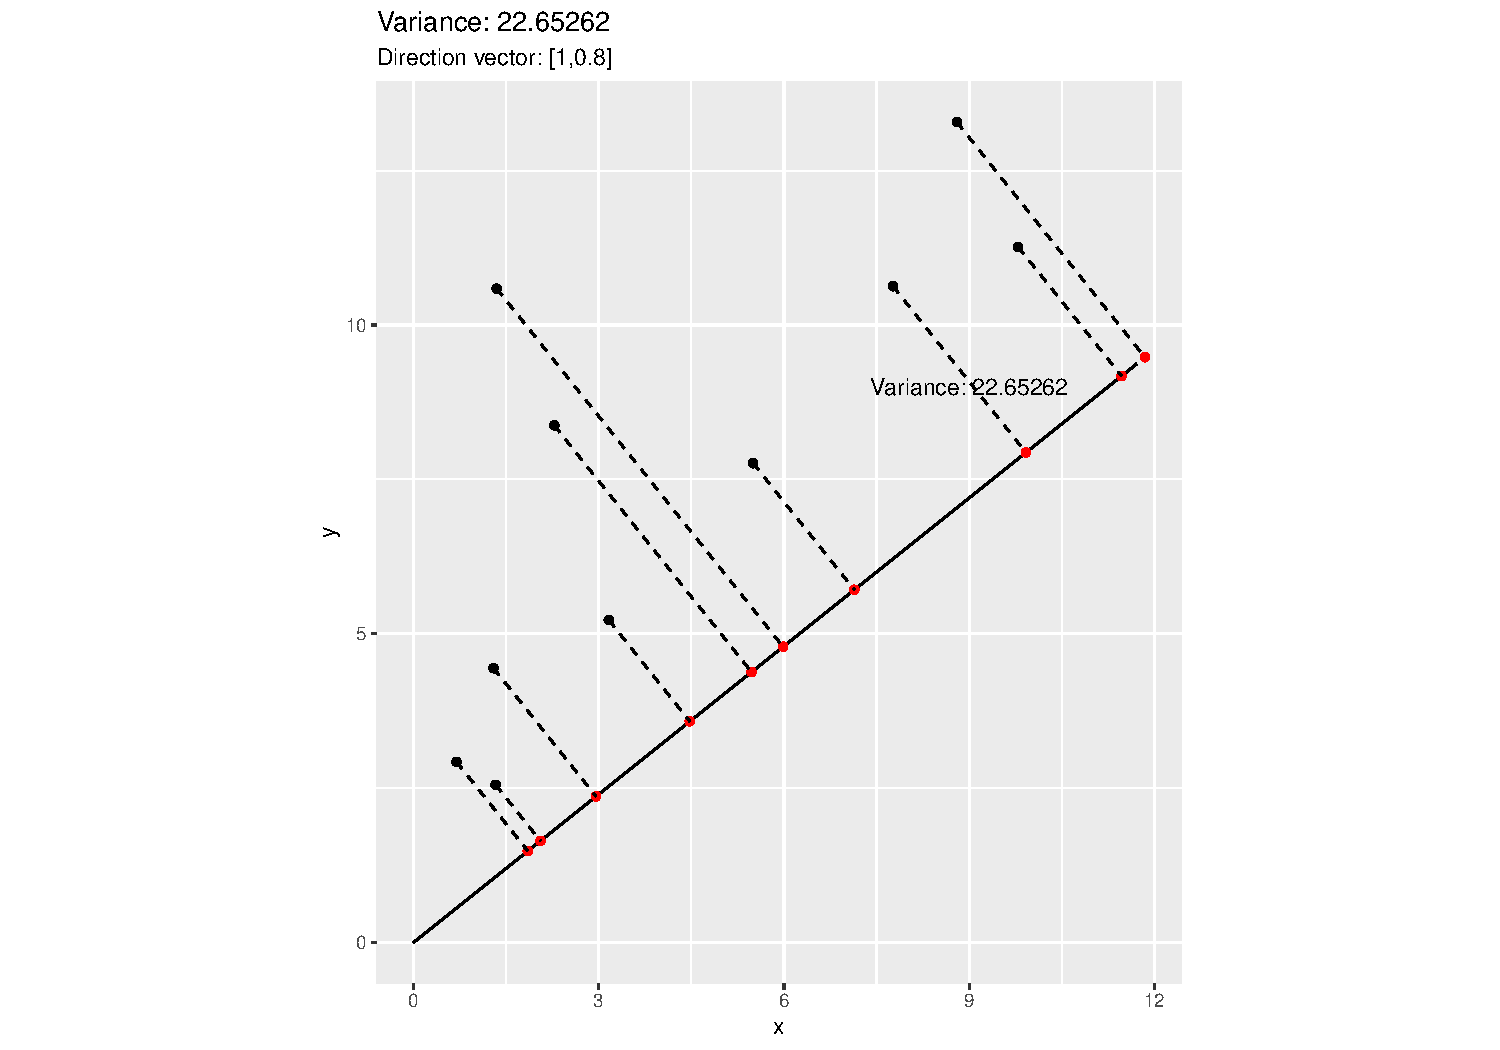
\includegraphics{note9_files/figure-beamer/unnamed-chunk-15-1.pdf}
\end{frame}

\begin{frame}{}
\protect\hypertarget{section-9}{}
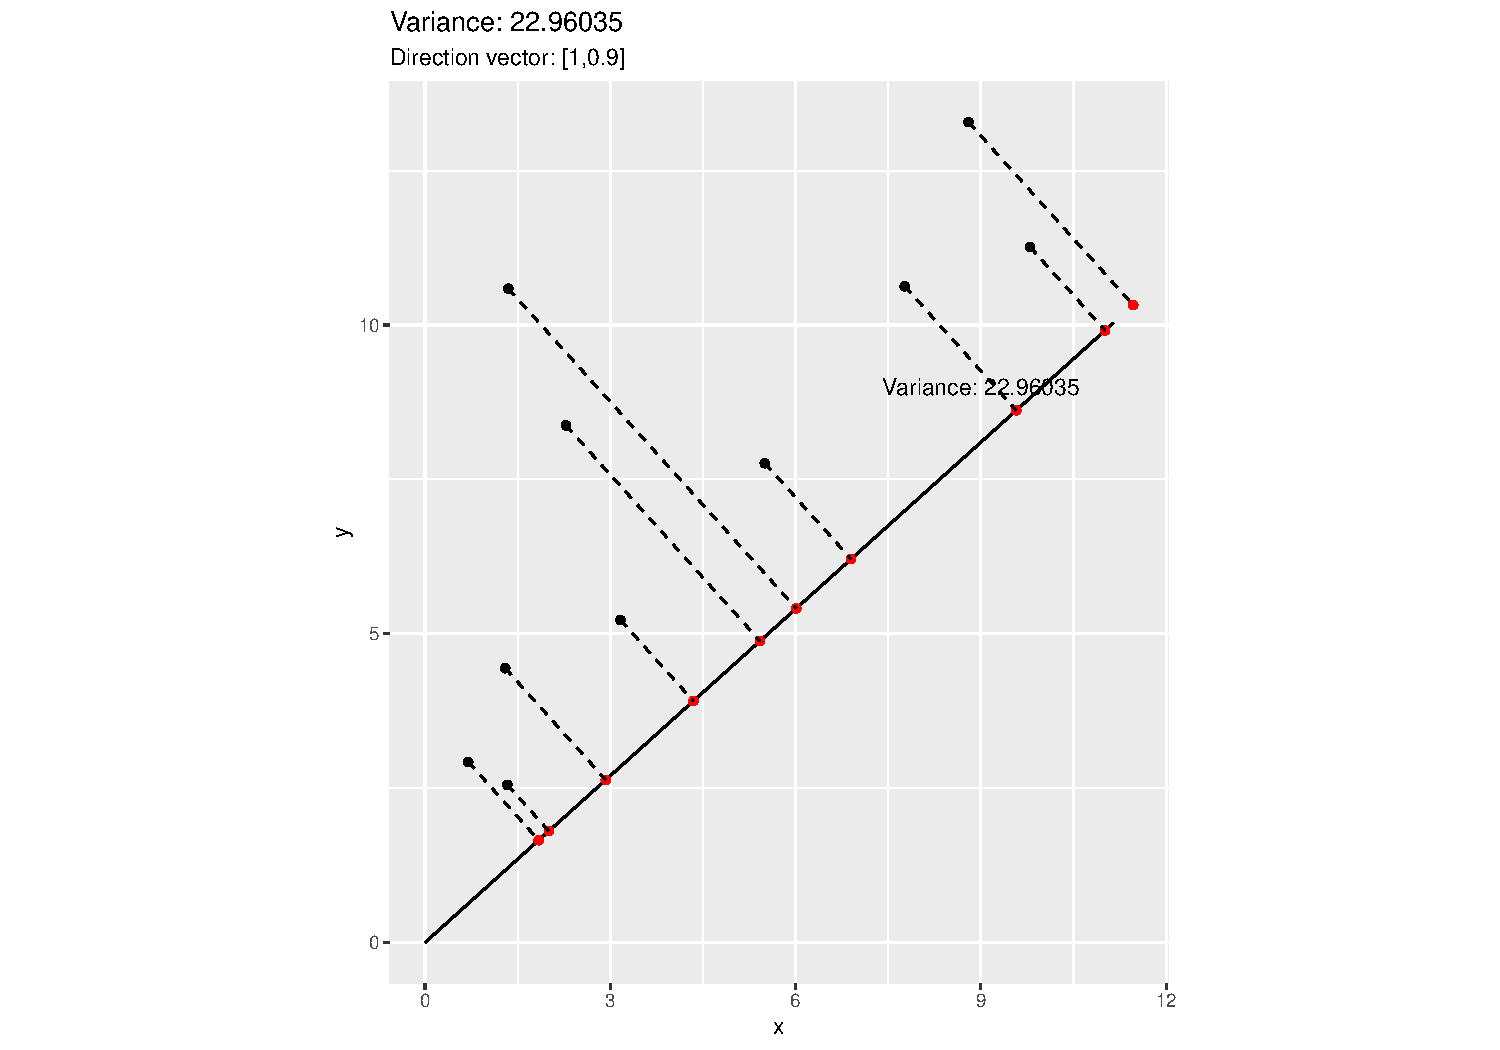
\includegraphics{note9_files/figure-beamer/unnamed-chunk-16-1.pdf}
\end{frame}

\begin{frame}{}
\protect\hypertarget{section-10}{}
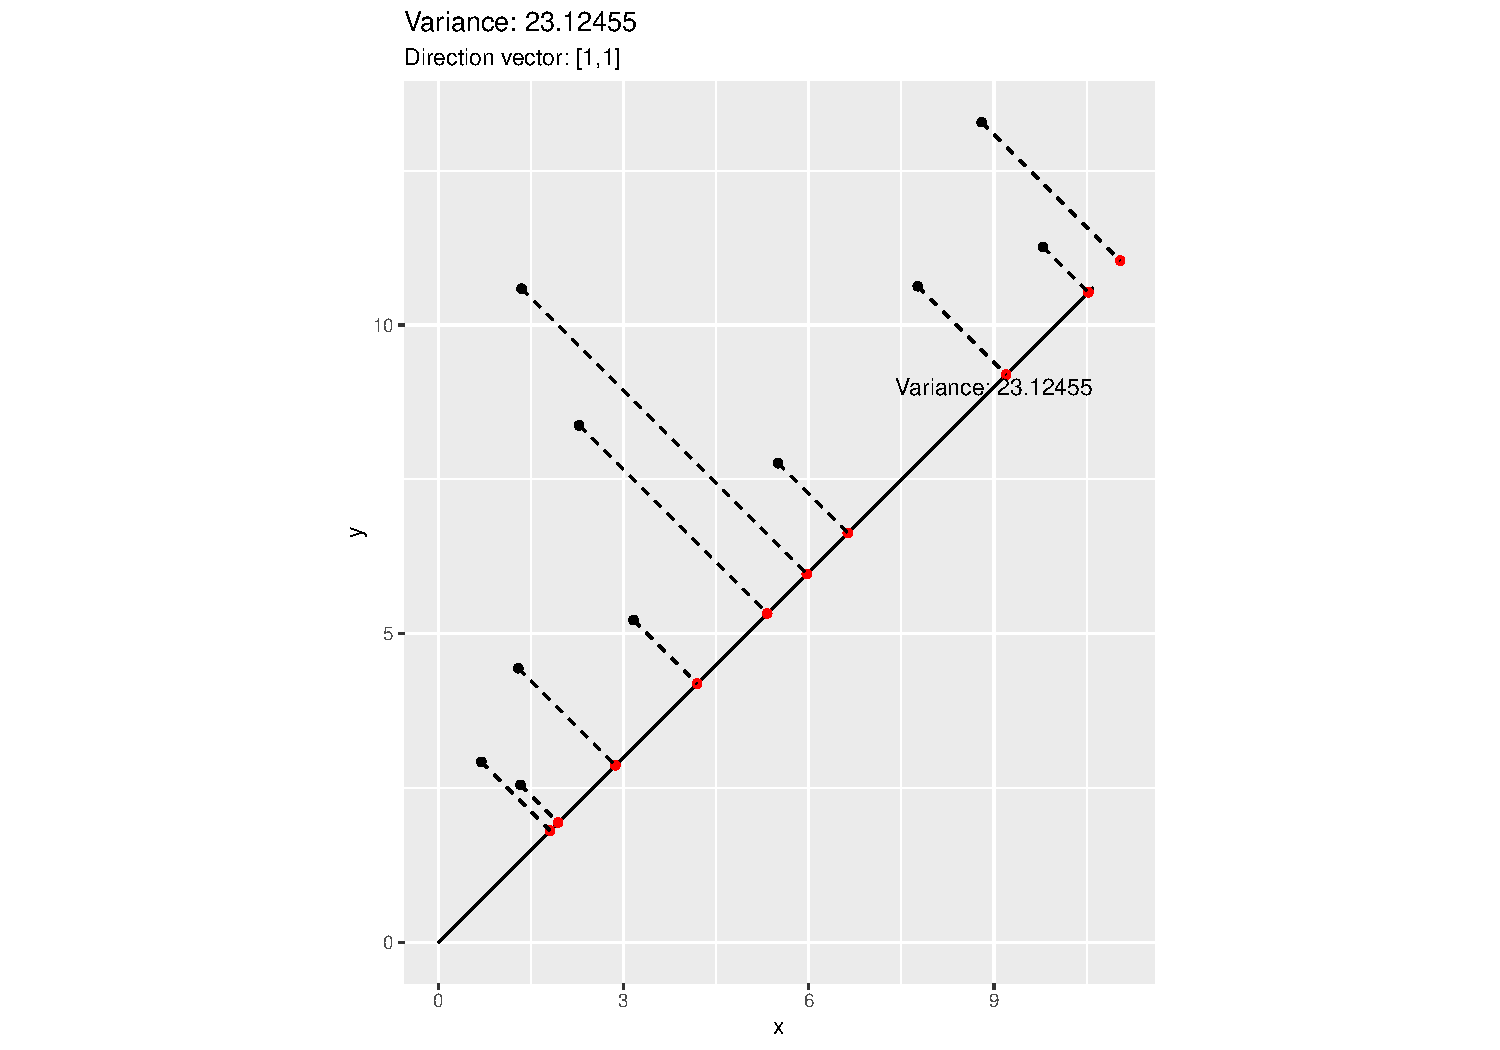
\includegraphics{note9_files/figure-beamer/unnamed-chunk-17-1.pdf}
\end{frame}

\begin{frame}{}
\protect\hypertarget{section-11}{}
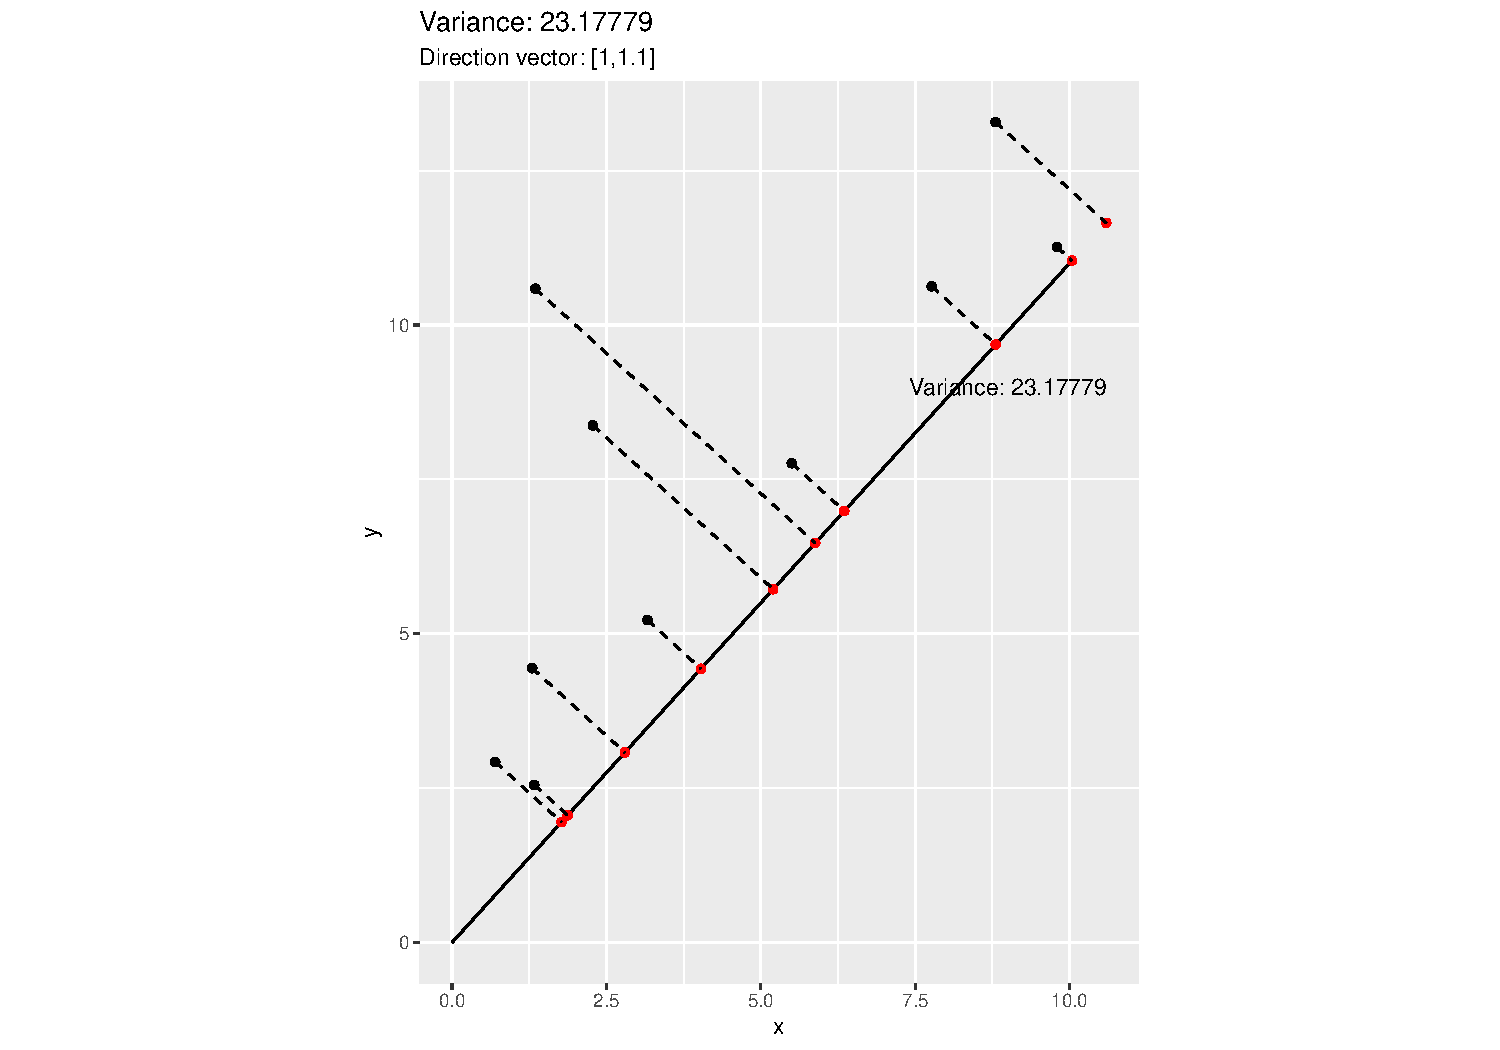
\includegraphics{note9_files/figure-beamer/unnamed-chunk-18-1.pdf}
\end{frame}

\begin{frame}{}
\protect\hypertarget{section-12}{}
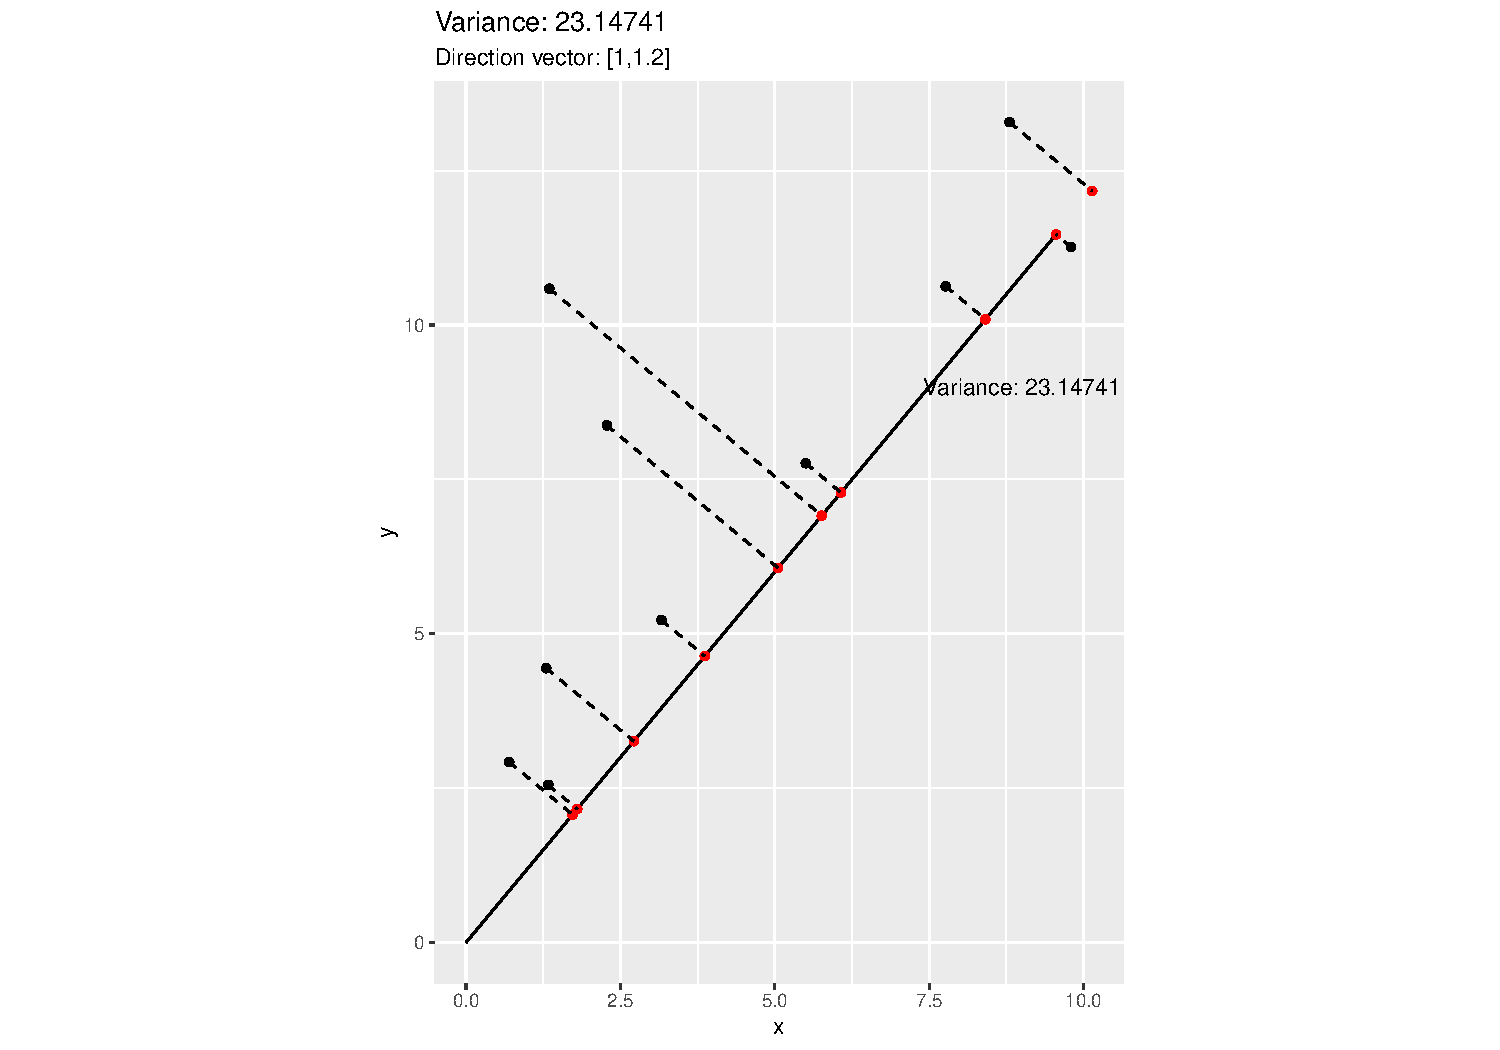
\includegraphics{note9_files/figure-beamer/unnamed-chunk-19-1.pdf}
\end{frame}

\begin{frame}{}
\protect\hypertarget{section-13}{}
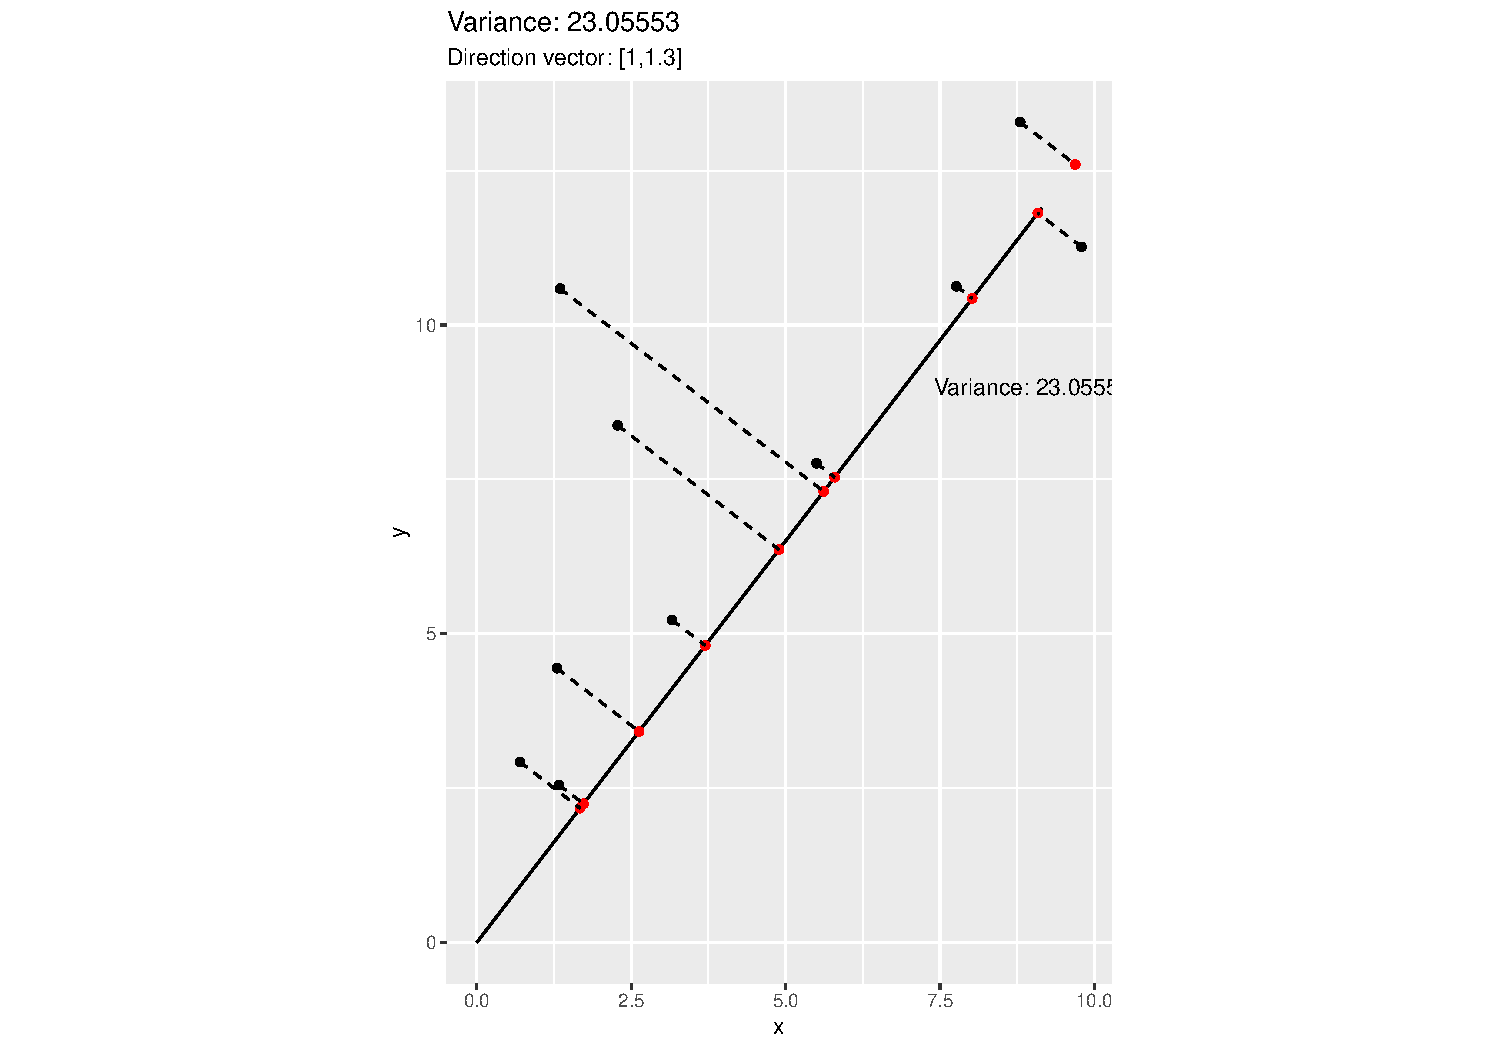
\includegraphics{note9_files/figure-beamer/unnamed-chunk-20-1.pdf}
\end{frame}

\begin{frame}{}
\protect\hypertarget{section-14}{}
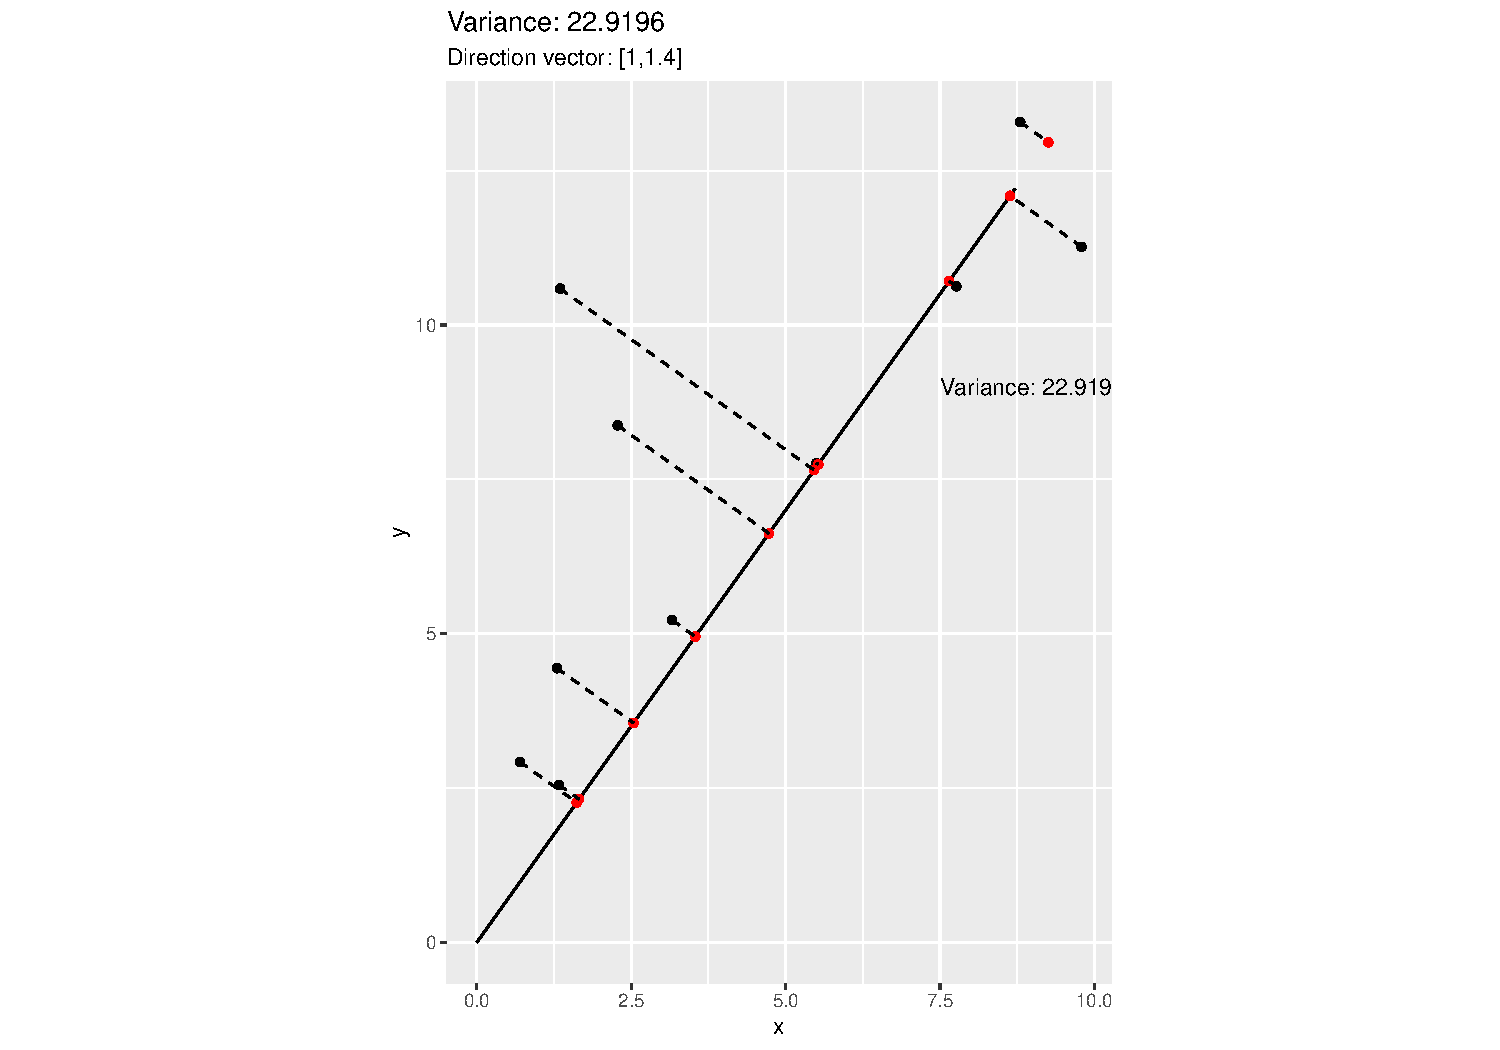
\includegraphics{note9_files/figure-beamer/unnamed-chunk-21-1.pdf}
\end{frame}

\begin{frame}{}
\protect\hypertarget{section-15}{}
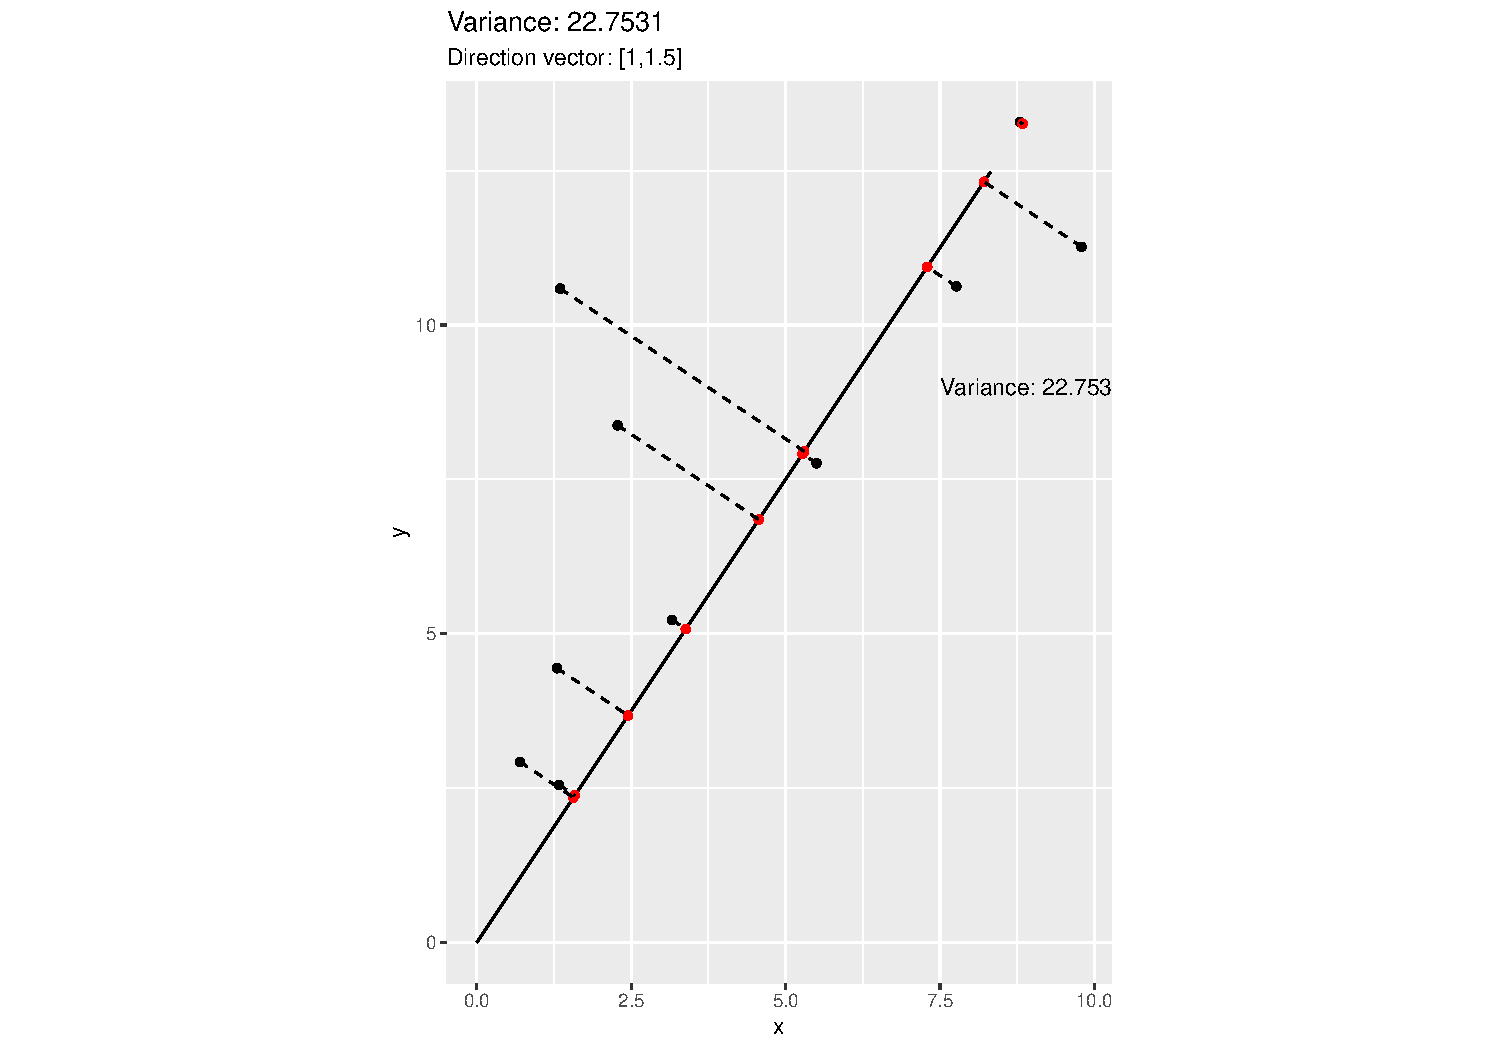
\includegraphics{note9_files/figure-beamer/unnamed-chunk-22-1.pdf}
\end{frame}

\begin{frame}{}
\protect\hypertarget{section-16}{}
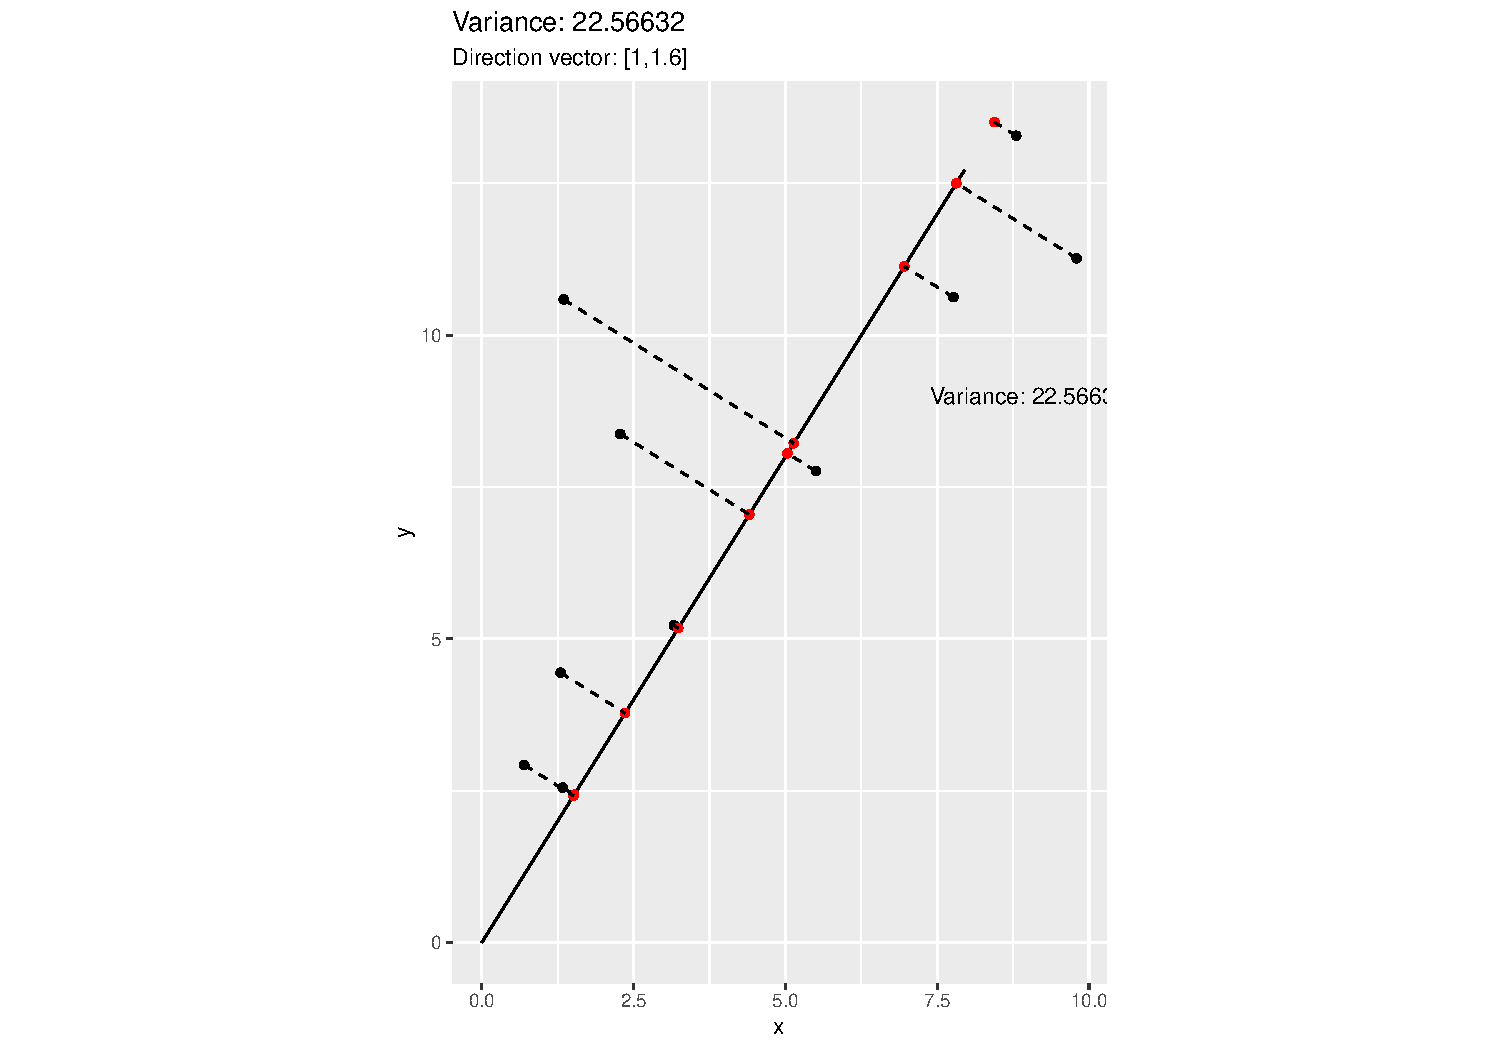
\includegraphics{note9_files/figure-beamer/unnamed-chunk-23-1.pdf}
\end{frame}

\begin{frame}{}
\protect\hypertarget{section-17}{}
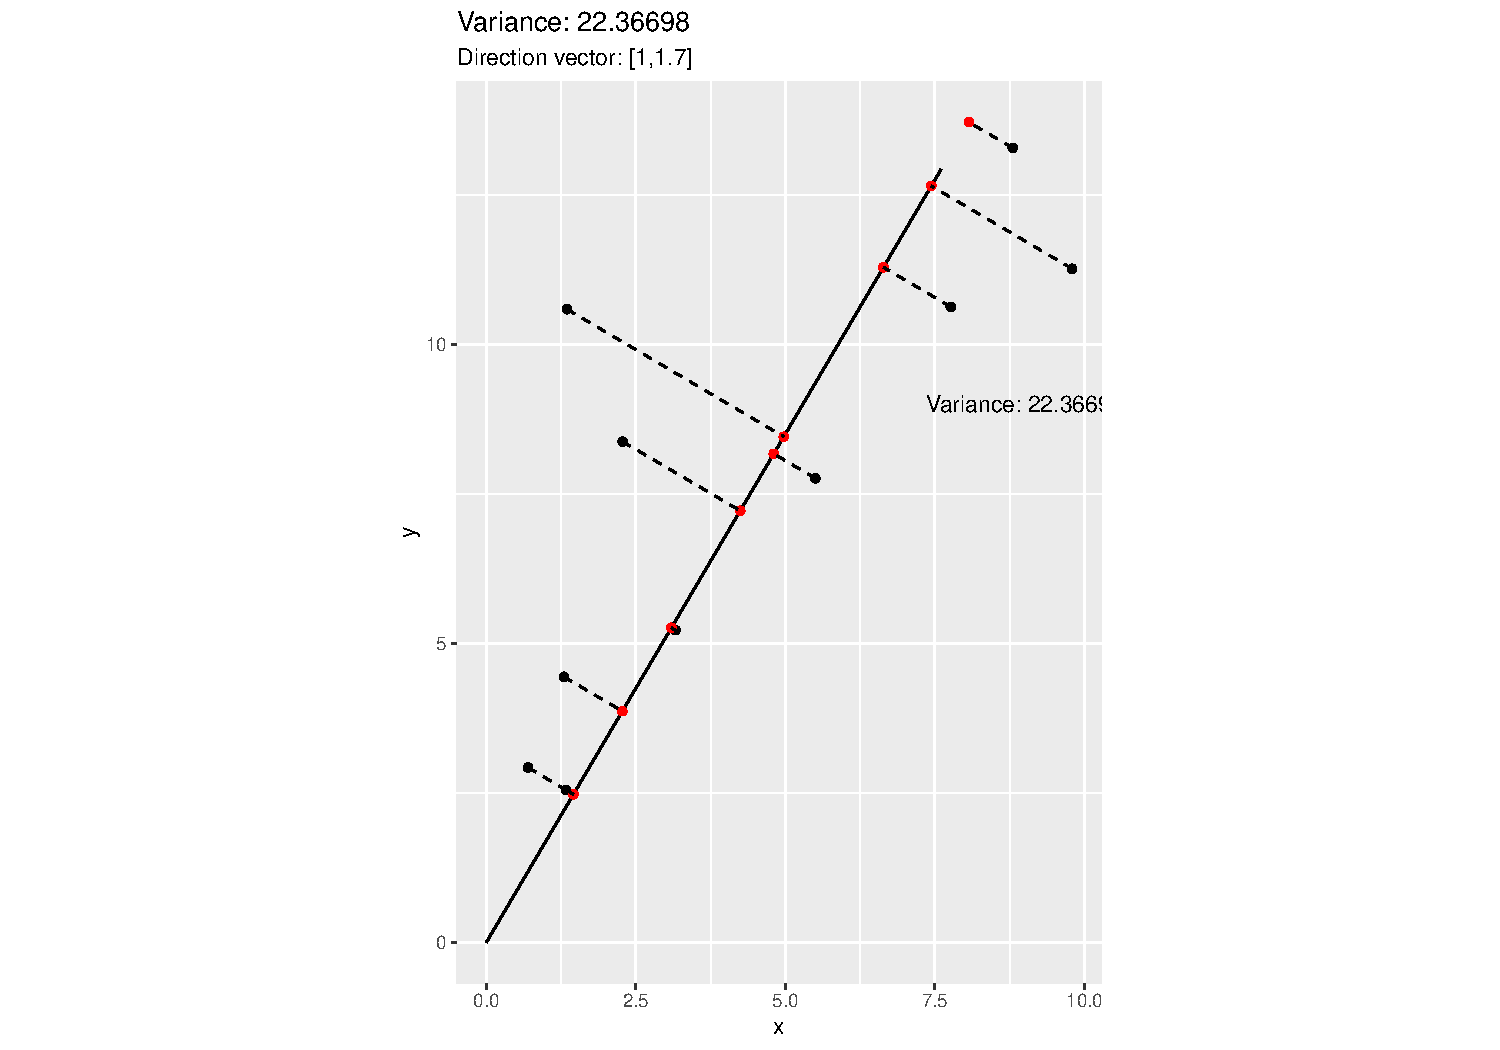
\includegraphics{note9_files/figure-beamer/unnamed-chunk-24-1.pdf}
\end{frame}

\begin{frame}{}
\protect\hypertarget{section-18}{}
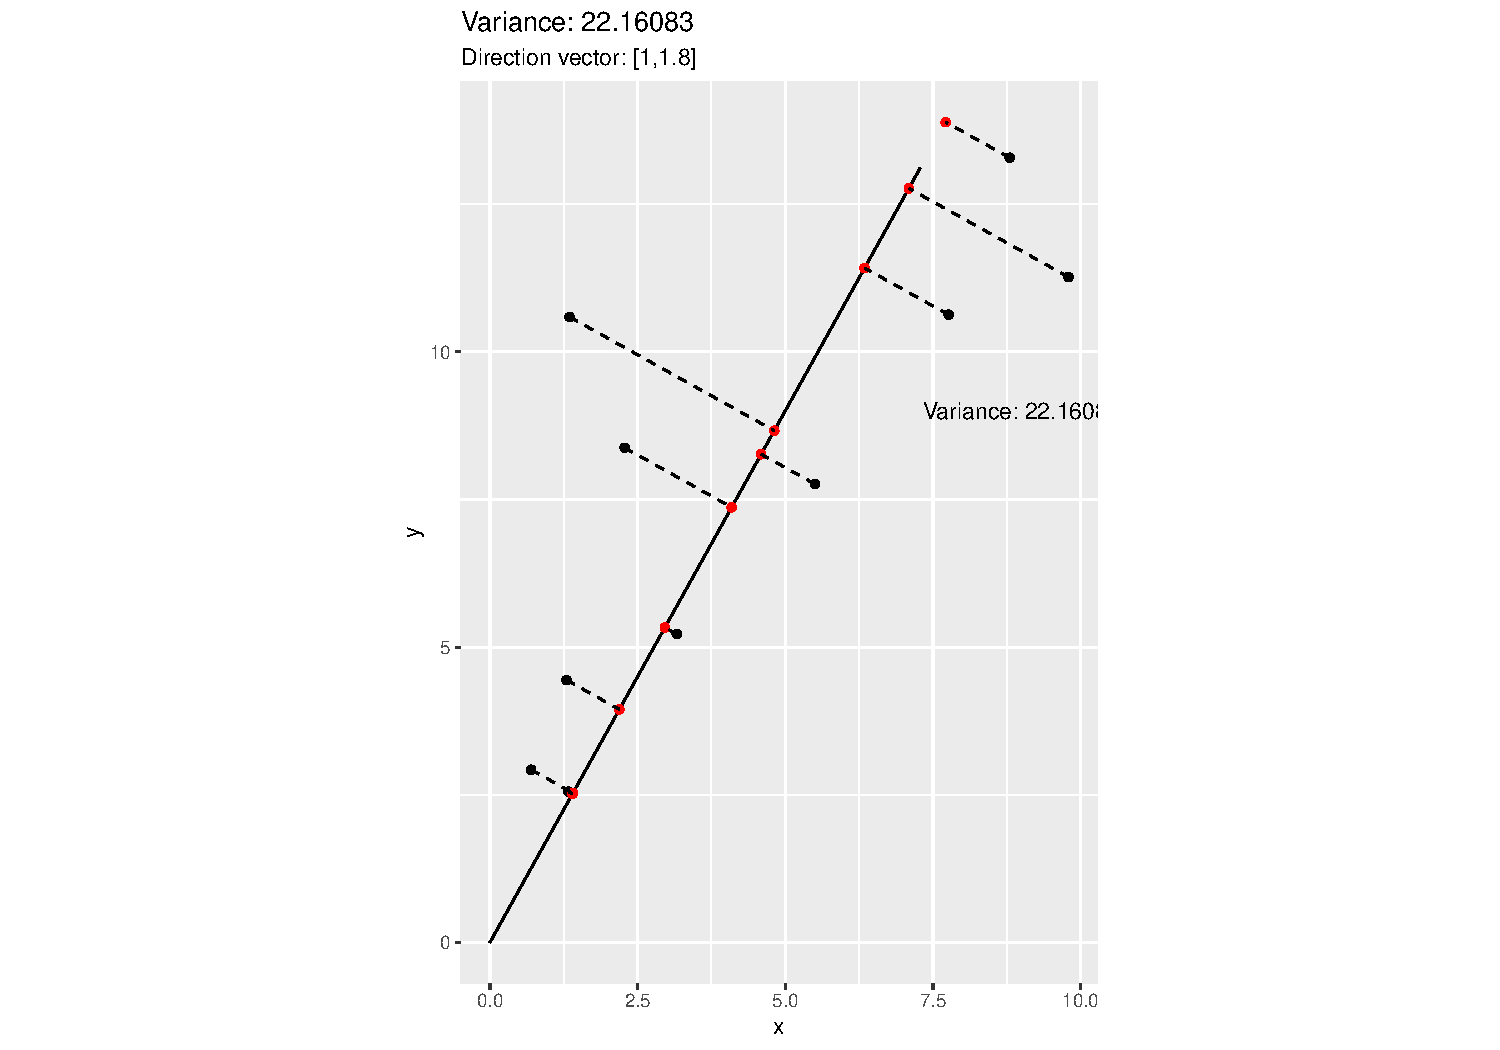
\includegraphics{note9_files/figure-beamer/unnamed-chunk-25-1.pdf}
\end{frame}

\begin{frame}{}
\protect\hypertarget{section-19}{}
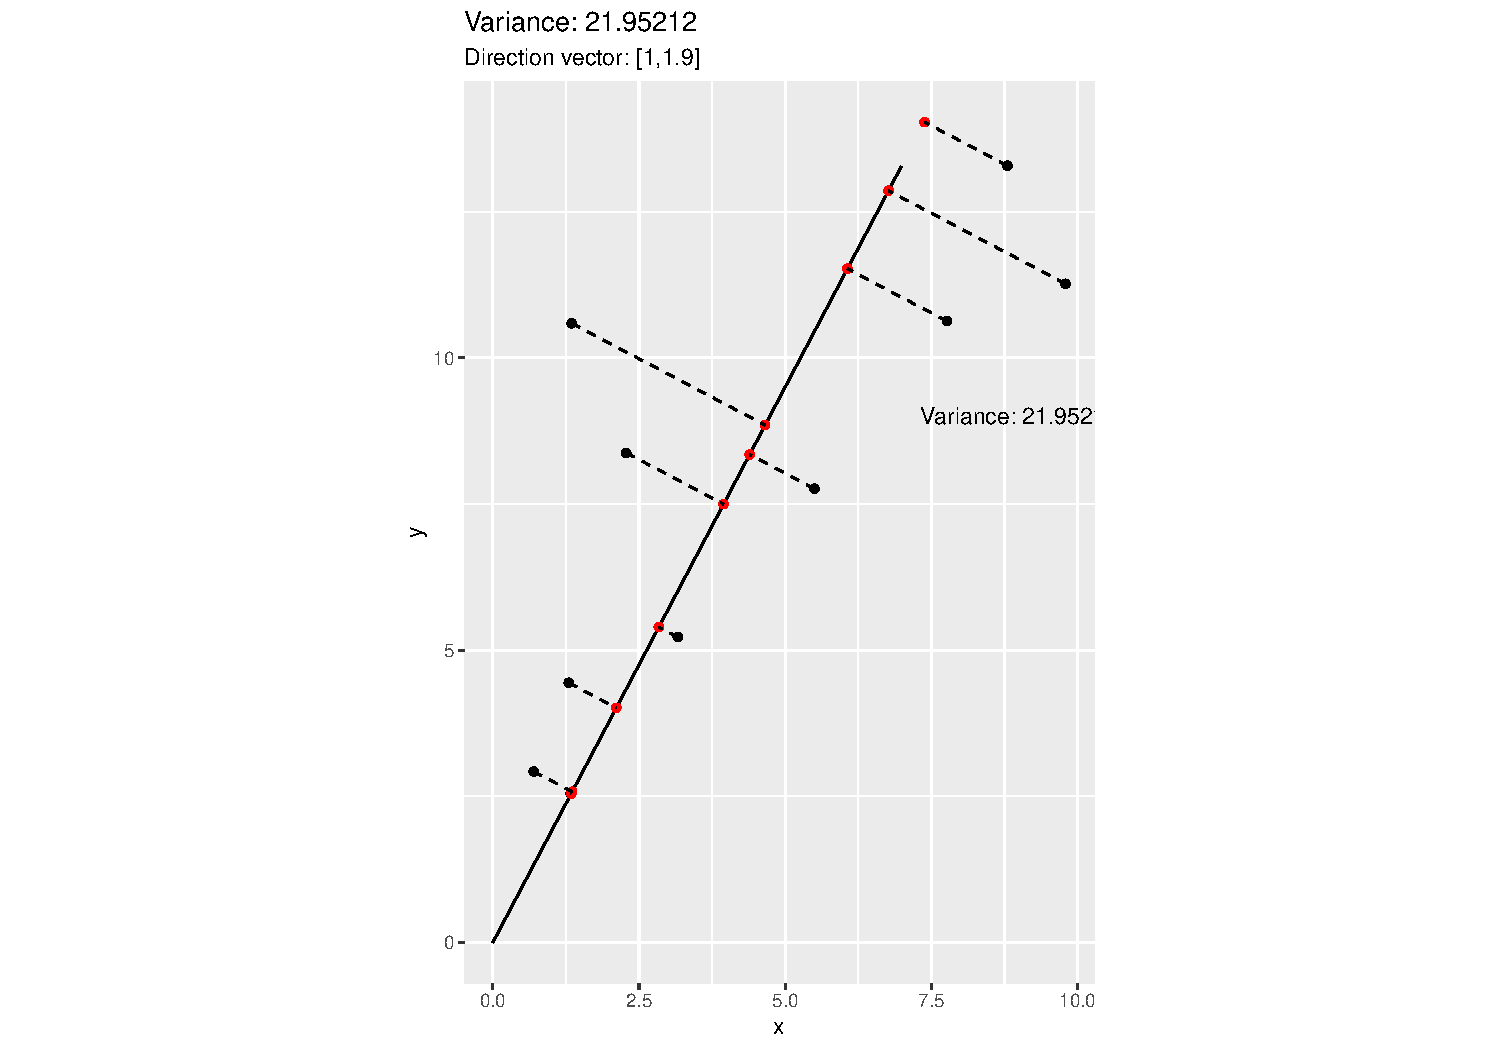
\includegraphics{note9_files/figure-beamer/unnamed-chunk-26-1.pdf}
\end{frame}

\begin{frame}{}
\protect\hypertarget{section-20}{}
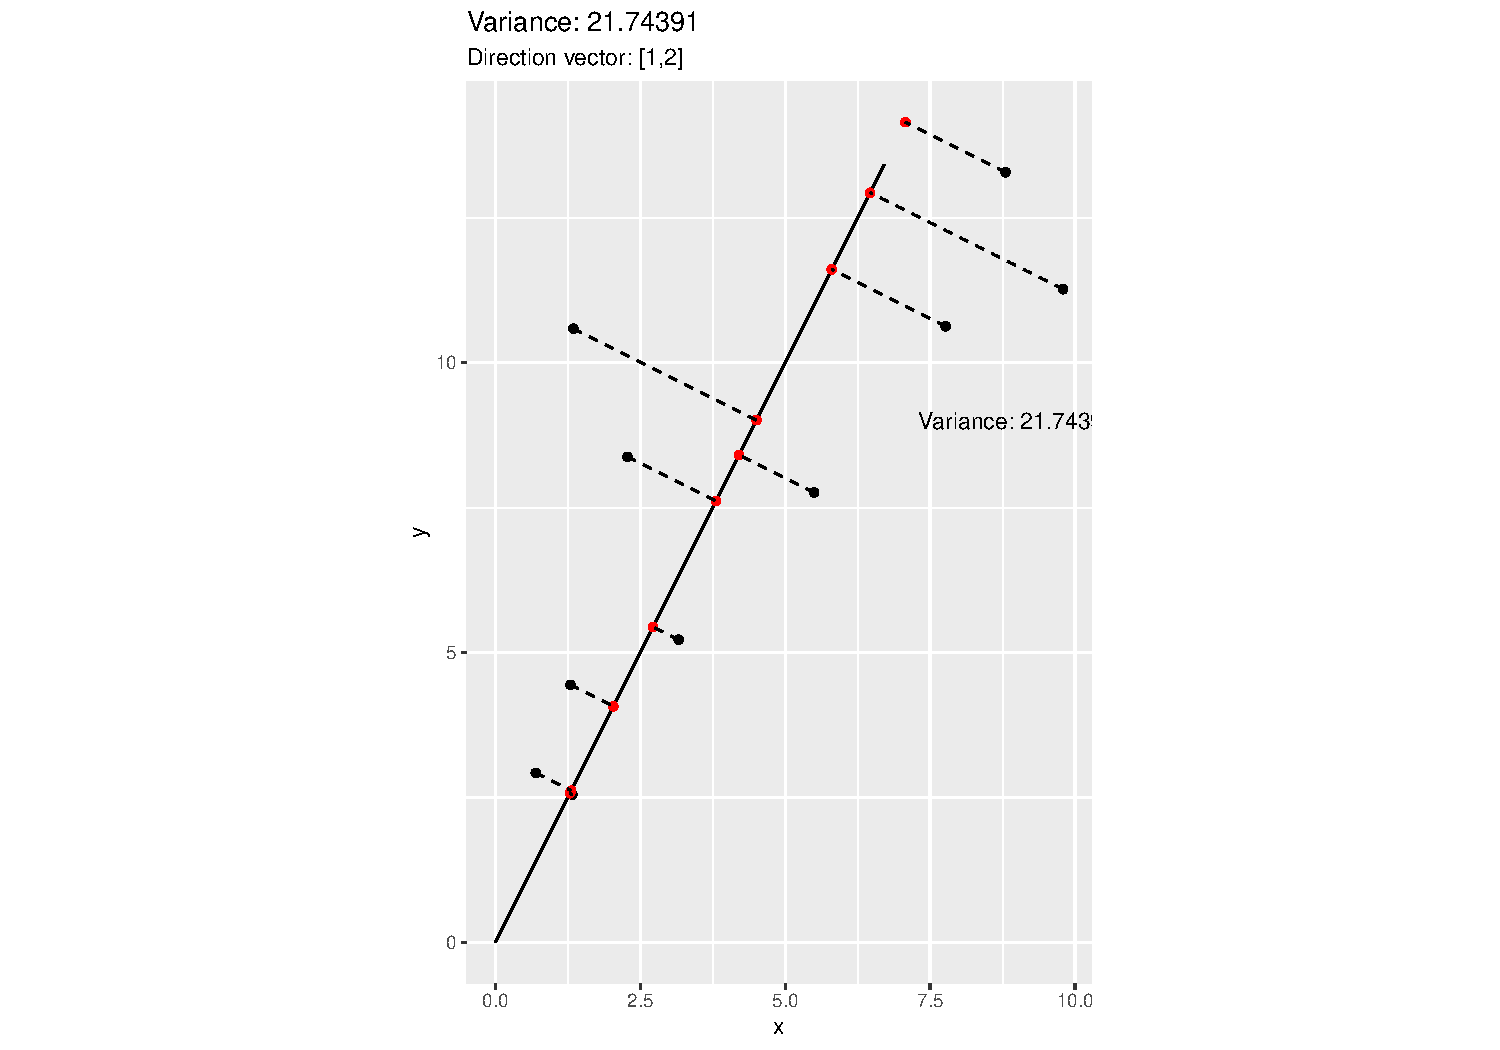
\includegraphics{note9_files/figure-beamer/unnamed-chunk-27-1.pdf}
\end{frame}

\begin{frame}{}
\protect\hypertarget{section-21}{}
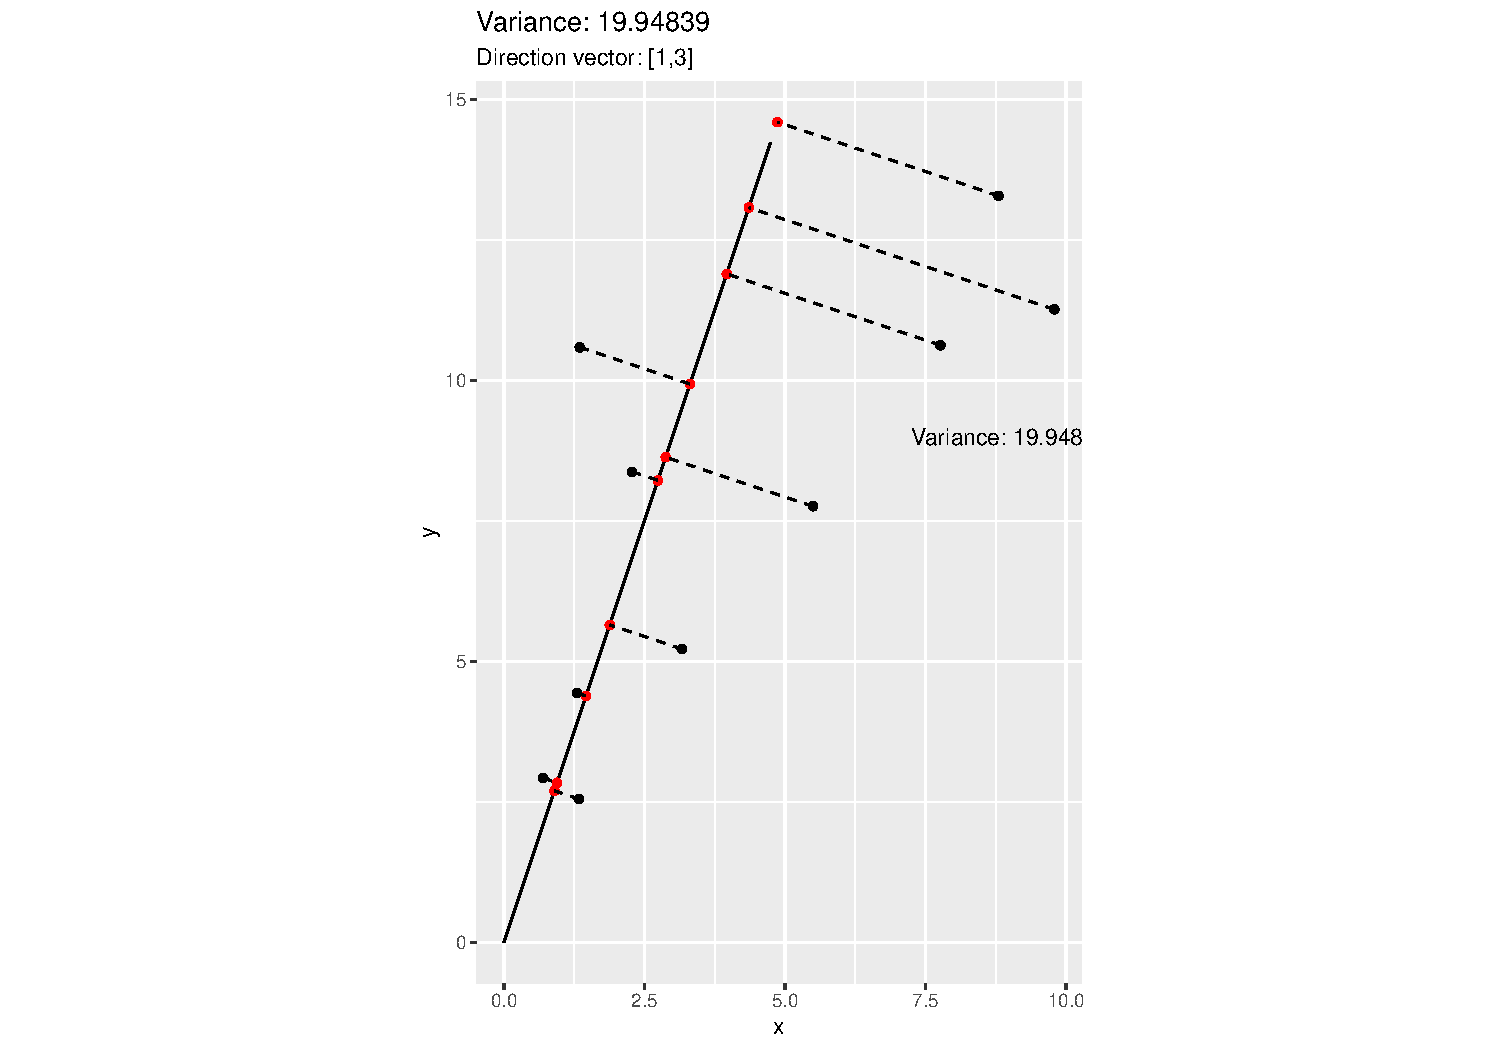
\includegraphics{note9_files/figure-beamer/unnamed-chunk-28-1.pdf}
\end{frame}

\begin{frame}{}
\protect\hypertarget{section-22}{}
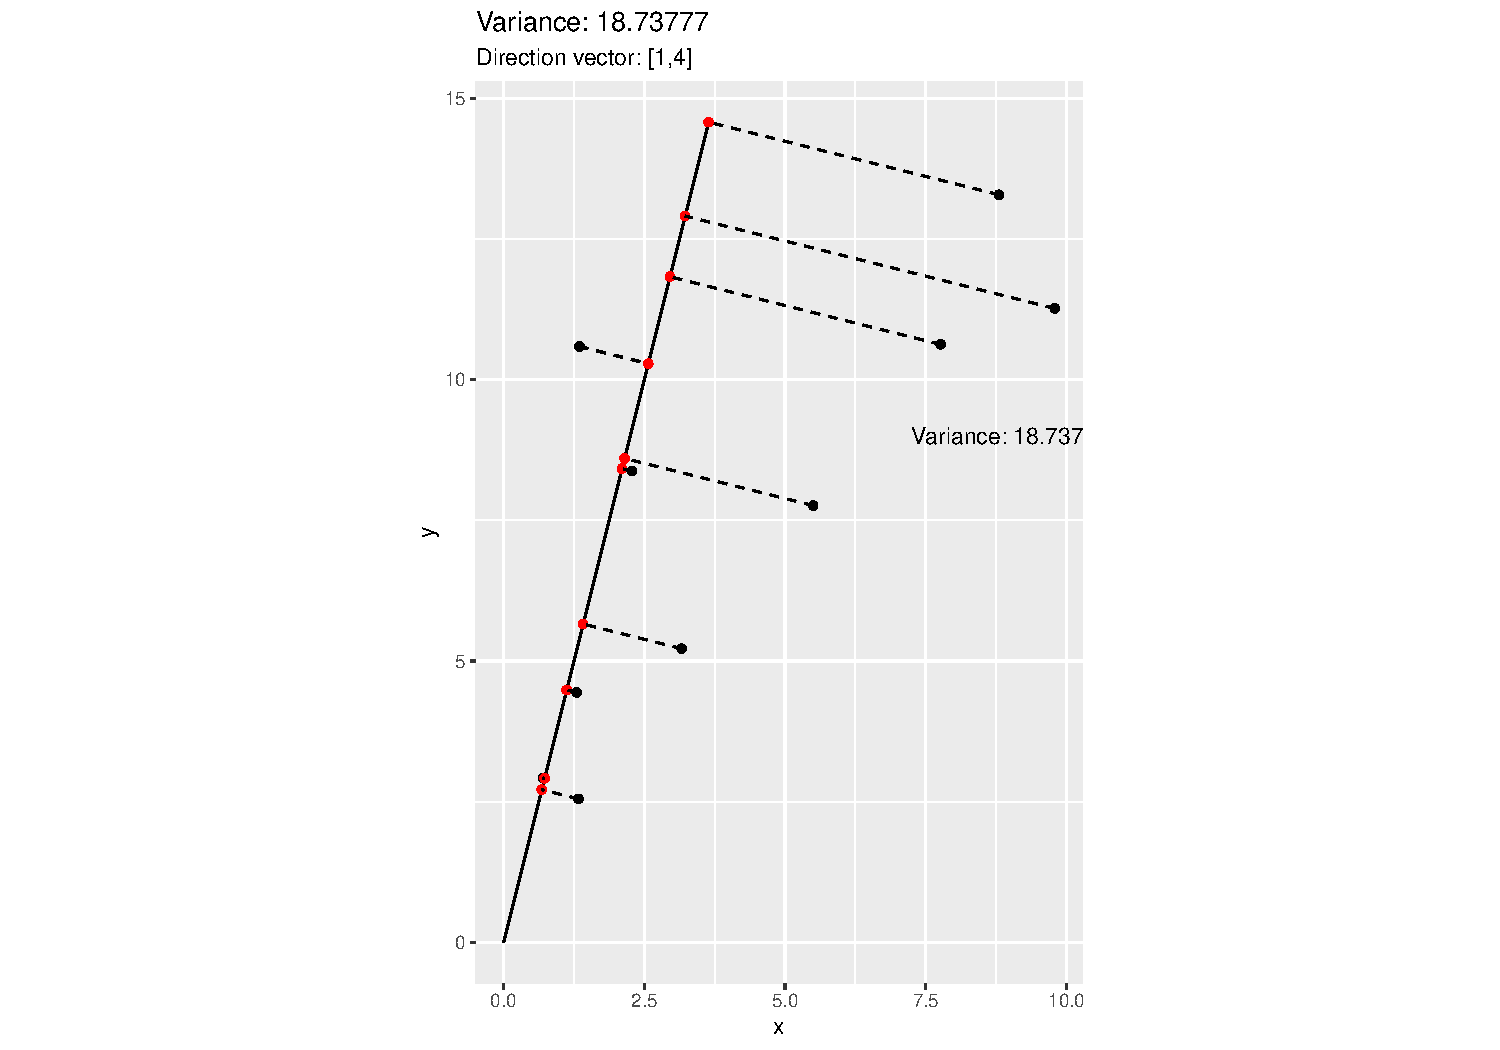
\includegraphics{note9_files/figure-beamer/unnamed-chunk-29-1.pdf}
\end{frame}

\begin{frame}{}
\protect\hypertarget{section-23}{}
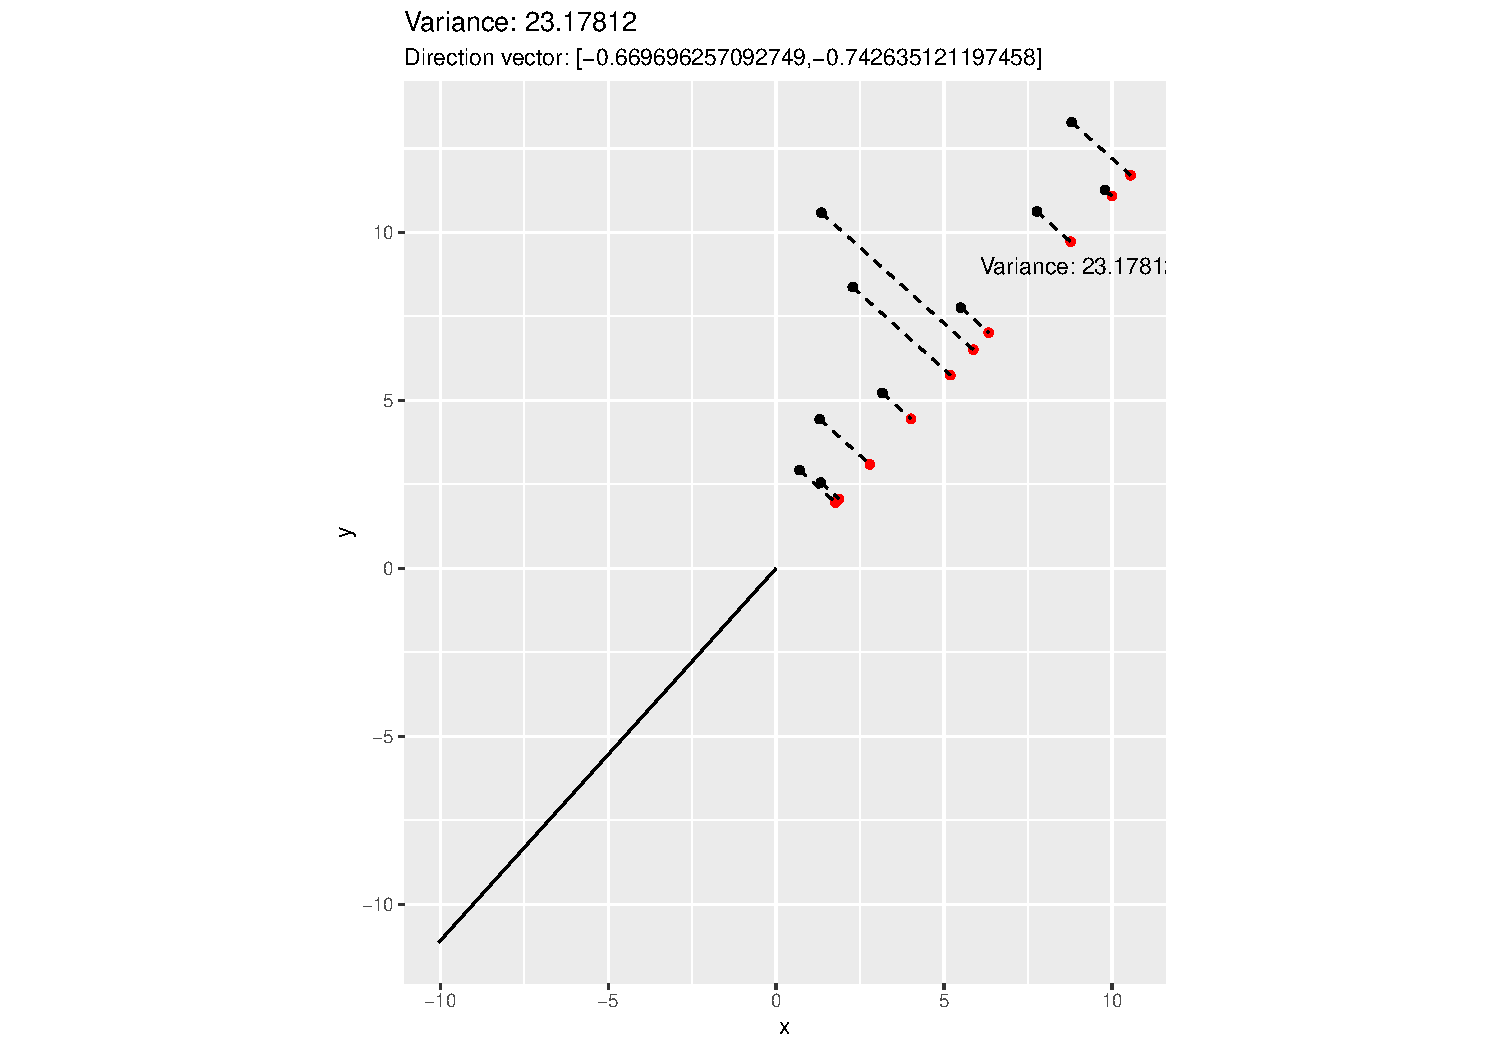
\includegraphics{note9_files/figure-beamer/unnamed-chunk-30-1.pdf}
\end{frame}



\end{document}
